%!TEX root = main.tex;

\documentclass[a4paper, oneside, 12pt]{report}
% \documentclass[12pt, a4paper, oneside]{memoir}
\usepackage[a4paper, inner=1.5cm, outer=3cm, top=2cm, bottom=3cm, bindingoffset=2cm]{geometry}

\usepackage[french]{babel}
% \usepackage{natbib}

% \usepackage[latin1]{inputenc}
\usepackage[T1]{fontenc}
\usepackage[utf8]{inputenc}
\usepackage{graphicx}
\usepackage{grffile}
\usepackage{verbatim}
\usepackage{float}
\usepackage{color}

\usepackage{titletoc}
%% enable styles for definitions
\usepackage{amsthm}
%% enable math
\usepackage{mathcomp}
\usepackage{amsmath}
%% for tabs
\usepackage{booktabs}
\usepackage{array}
% \usepackage{standalone}
% \usepackage{tikz}
\usepackage{amsmath}
\usepackage{amssymb}
\usepackage{hyperref}
\usepackage{blindtext}
\usepackage{url}
\usepackage{titlesec}
\usepackage{lmodern}
\usepackage{fancyvrb}

\usepackage{caption}
\usepackage{subcaption}
\usepackage[toc,page]{appendix}
\renewcommand{\appendixpagename}{Annexes}
\renewcommand{\appendixtocname}{Annexes}


\setcounter{secnumdepth}{5} 
\linespread{1.5}

\usepackage[acronym]{glossaries}

\usepackage[outdir=./]{epstopdf}
\makeglossaries

\author{TAOURIRIT Salah Eddine}
\title{composition des services web}

\date{\today\\version 0.2.4}
\begin{document}

%description style
\let\Item\item
\newcommand{\head}[1]{\textnormal{\textbf{#1}}}
\newcommand\SpecialItem{\renewcommand\item[1][]{\Item[\textbullet~\sffamily ##1]}}
\newcommand\SpecialItemi{\renewcommand\item[1][]{\Item[\textendash~\sffamily ##1]}}
\renewcommand\enddescription{\endlist\global\let\item\Item}
% enable it if you want an arabic numeration for subsubsubsection
% \renewcommand{\thesubsubsection}{\arabic{subsection}.\alph{subsubsection})}
\renewcommand{\descriptionlabel}[1]{\hspace{1cm}\textsf{#1}} 
\newtheorem{mydef}{Definition}

\maketitle 

\setcounter{secnumdepth}{4}
\setcounter{tocdepth}{4}
\selectlanguage{french}  

\pagenumbering{roman}
\tableofcontents
\newacronym{xml}{XML}{Extensible Markup Language}
\newacronym{soap}{SOAP}{Simple Object Access Protocol}
\newacronym{wsdl}{WSDL}{Web Services Description Language}
\newacronym{uddi}{UDDI}{Universal Description Discovery and
Integration} \newacronym{w3c}{W3C}{The World Wide Web Consortium}
\newacronym{http}{HTTP}{Hypertext Transfer Protocol}
\newacronym{sawsdl}{SAWSDL}{Semantic Annotations for WSDL and XML
Schema} \newacronym{wsmo}{WSMO}{Web service modeling ontology}
\newacronym{wsml}{WSML}{web service modeling language}
\newacronym{swsf}{SWSF}{Semantic web services framework}
\newacronym{daml}{DAML}{the DARPA Agent Markup Language}
\newacronym{darba}{DARBA}{Defence Advanced Research Projects Agency}
\newacronym{bpel}{BPEL}{Business Process Execution Language}
\newacronym{ws-bpel}{WS-BPEL}{Web Service Business Process Execution
Language} \newacronym{bpel4ws}{BPEL4WS}{Business Process Execution
Language for Web Services} \newacronym{xlang}{XLANG}{XML Business
Process Language} \newacronym{wsfl}{WSFL}{Web Services Flow Language}
\newacronym{wsci}{WSCI}{Web Service Choreography Interface}
\newacronym{ws-cdl}{WS-CDL}{Web Services Choreography Description
Language} \newacronym{wsmf}{WSMF}{The Web Service Modeling Framework}
\newacronym{qos}{QoS}{Quality of service} \newacronym{mdo}{MDO}{Model
driven engineering} \newacronym{sws}{SWS}{synthesized Web services}
\newacronym{uml}{UML}{Unified Modeling Language}
\newacronym{ccs}{CCS}{Calculus of Communicating Systems}
\newacronym{csp}{CSP}{Communicating Sequential Processes}
\newacronym{json}{JSON}{JavaScript Object Notation}
\newacronym{nosql}{NoSQL}{Not Only SQL}
\newacronym{SGBD}{SGBD}{Système De Gestion Des Bases de Données}
\newacronym{SGBDR}{SGBDR}{Système De Gestion Des Bases de Données Relationnelles}
\newacronym{DSL}{DSL}{Domain Specific Language}

\printglossaries
\listoffigures
\listoftables

\pagenumbering{arabic}
%!TEX root = ../main.tex

\section{Introduction}
Dans le domaine des services web, il y'a plusiers méthode de la composition des 
services web.\\


\part{Étude bibliographique}
% !TEX root = ../main.tex < 20 pages

% \chapter{Concepts de base du paradigme service Web}
% Une introduction implicite du chapitre %TODO
% Dans ce chapitre on va faire une vue générale sur les technologies
% des services web sémantiques, Pour bien introduire le chapitre
% prochain sur la composition des services web.

\chapter{Les services web: Vue d'ensemble}

Ce chapitre établit une étude du fondement théorique de notre travail à savoir les concepts de base 
du paradigme service Web.  Nous commençons d'abord par présenter un tour d'horizon définissant l'architecture
de référence de ce paradigme ainsi que quelque définitions proposées par la littérature. Ensuite nous nous
intéressons à montrer les limitation de l'approche syntaxique de la description des services web et 
l'apport de l'enrichissement sémantique de cette dernière aux processus de la découverte et la composition 
des services Web.\\
  % TODO: complete the introduction
\newpage

  \section{Notions de base et technologies associées} 

  Les services Web constituent une approche pour mettre en œuvre le paradigme de service,
  et peut être vue comme une instance de l'architecture orienté service.

  Dans cette section va parler aussi d'un socle technologique très sollicité, On va aussi Détailler 
  l'architecture de base d'un service web, ensuite nous introduisons l'architecture étendus.


    \subsection{Définitions et caractéristiques }
    Les services Web sont la technologie la plus connue et la plus populaire dans le monde 
    industriel et académique pour la mise en place d’architectures à services.

    % ARE PROGRAMMABLE COMPONENTS which use the World- Wide-Web as a
    % medium for describing the functionality of real world ser- vices in
    % a computer manipulable way (Kuropka and Nern, 2006)
    Les Web services ont été proposés initialement par IBM \cite{kreger2001web} et Microsoft, puis en
    standardisés par le \acrshort{w3c} \footnote{\url{http://www.w3.org/}} et définis \cite{WSA} par :\\


    \emph{``Un service web est un système conçu pour permettre
      d'interopérabilité des applications à travers un réseau.  Il est
      caractérisé par un format de description
      interprétable/compréhensible automatiquement par la machine,
      D'autres systèmes peuvent interagir avec le Service Web selon la
      manière prescrite dans sa description et en utilisant des messages
      SOAP, généralement transmis via
      le protocole HTTP et sérialisés en XML et en d'autres standards du Web ''}.\\

    Cette définition surligne les caractéristiques clés de services Web
    \cite{fremantle2002enterprise}:

    \SpecialItem
    \begin{description} % Les caractéristiques des services web Selon la définition de W3C
    \item[Basés sur des protocoles Internet] : L'utilisation de
      \acrshort{http} pour le transport des informations permet de
      traverser les contrôles d'accès dans un environnement hétérogène.
  
    \item[Interopérables] : Le standard \textsc{SOAP} \cite{box2000simple}
      définit comme étant un protocole destiné à l'échange de messages
      structurés véhiculé généralement sur \acrshort{http} et sérialisé en
      \textsc{XML}, permettant le support pour l'interopérabilité.
      
    \item[Basés sur XML] : Le méta-langage de balisage \textsc{XML}
      \textit{eXtensible Markup Language} est un standard Web ouvert par
      \textsc{W3C} \cite{bray1998extensible} offre un cadre standard pour
      la définition de documents Interprétable par des machines.
    \end{description}
    
    M. P. Papazoglou \cite{papazoglou2003service} apporte une autre définition de services web:\\
    \emph{``Les services Web sont des éléments auto-descriptifs et
      indépendants des plateformes permettent la composition faible coût
      d’applications distribuées. Les services Web effectuent des
      fonctions allant de simples requêtes des processus métiers
      complexes. Les services Web permettent aux organisations d’exposer
      leurs programmes résultats sur Internet (ou sur un intranet) en
      utilisant des langages (basés sur XML) et des protocoles
      standardisés et de les mettre en œuvre via une interface
      auto-descriptive basée sur des formats standardisés et ouverts''}
    % TODO make a comment on this def and introduce the web services
    % composition idea !
    
    
    % TODO organize this mess * Permettre l'interopéabilité des
    % applications, indépendamment des plates-formes et des langages
    
    % * Permettre le couplage faible des applications (évolution
    % indépendante) et leur coopération via des interfaces de haut niveau
    % d'abstraction (services globaux)
    
    % * Permettre une coopération des applications avec un minimum
    % d'intervention humaine
    Curbera et al. \cite{curbera2001web} de ça part proposent la définition suivante :\\
    
    \emph{``Un service Web est une application réseau capable d'interagir
      par le moyen des standards et des protocoles via des interfaces bien
      spécifiés, dans lequel est décris utilisant un langage de
      description fonctionnel
      standardisé''}.\\

    % Brièvement, un service Web est une entité logiciel modulaire,
    % auto-descriptive et autonome accessible via Internet.
    
    \subsection{L'évolution des styles des services web}
    % Les architecture communes des services web SOAP vs REST les limites
    % de la'approche SOAP pourquoi SOAP pour notre problème?
    ``the next section provides a short history of web services, with
    emphasis on the kinds of software challenges that web services are
    meant to address.''
    
    \subsection{L'architecture de référence et technlogies associées}
    \cite{curbera2002unraveling} \cite{gottschalk2002introduction}
    \cite{kreger2001web} \cite{WSA}
    % The basic SOAP/WSDL/UDDI standards are a particular implementation
    % of the concept of a service- oriented architecture.  cette
    % sous-section va détaillé SOAP et pas de WSDL et UDDI
    Cette architecture a été proposée afin de promouvoir
    l’interopérabilité et l’extensibilité des services Web Dans
    l'ensemble, une architecture complète de services Web est constitué
    d'un fournisseur de servicee \footnote{Providers}, un annuaire de
    services \footnote{Service Registry}, et un client
    \footnote{Service Requester} de service.  La figure x montre comment ces trois rôles interagissent.\\

    \SpecialItem
    \begin{description} % TODO tranlate: Les Rôles dans une architecture WSA
    \item[Le fournisseur] A service provider provides the interface for
      the Web service and the implementation of the application. The
      service provider is also responsible for creating the definition of
      the service and publishing that definition to meet the Universal
      Description, Discovery, and Integration (UDDI) specification.
  
    \item[L'annuaire] A service registry is a way in which Web services
      are formally published. The service registry is based on the UDDI
      specification and reflects information about services provided by
      the service provider. The service registry provides a service
      requester with a Web Services Description Language (WSDL) service
      description and a Uniform Resource Locator (URL) that points to the
      service itself.
  
    \item[Le client] A service requester is the consumer of a Web service
      and uses the service registry to gain information about, and access
      to, a Web service.
      
    \end{description}

    For an application to take advantage of Web Services, three behaviors
    must take place: publication of service descriptions, lookup or
    finding of service descriptions, and binding or invoking of services
    based on the service description. These behaviors can occur singly or
    iteratively. In detail, these operations are: \SpecialItem
    \begin{description}% TODO tranlate: WS actions
    \item[Publish] To be accessible, a service description needs to be
      published so that the service requestor can find it. Where it is
      published can vary depending upon the requirements of the
      application (see “Service Publication” for more details).
  
    \item[Find] In the find operation, the service requestor retrieves a
      service description directly or queries the service registry for the
      type of service required (see “Service Discovery” for more
      details). The find operation can be involved in two different
      lifecycle phases for the service requestor: at design time to
      retrieve the service’s interface description for program
      development, and at runtime to retrieve the service’s binding and
      location description for invocation.
      
    \item[Bind] Eventually, a service needs to be invoked. In the bind
      operation the service requestor invokes or initiates an interaction
      with the service at runtime using the binding details in the service
      description to locate, contact and invoke the service.
    \end{description}

    % \begin{description} % SOAP + WSDL + UDDI
    Les services Web sont construits autour de standards qui sont
    \acrshort{soap}, \acrshort{wsdl} et \acrshort{uddi} assurant
    respectivement leur communication, leur description et leur découverte.

      \subsubsection{Communication: SOAP}
      Développé par IBM\footnote{\url{http://www.ibm.com}} et
      Microsoft\footnote{\url{http://www.microsoft.com}}
      \cite{box2000simple}, L'approche \textsc{SOAP} est une recommandation \textsc{W3C} qui le
      définit comme étant un protocole destiné à l'échange de messages
      structurés, permettant d'invoquer des applications sur des réseaux
      distribués \cite{mitra2003soap}.\\   
      \begin{figure}[htbp]
    \centering
    \begin{subfigure}[b]{1\textwidth}        
	\centering
	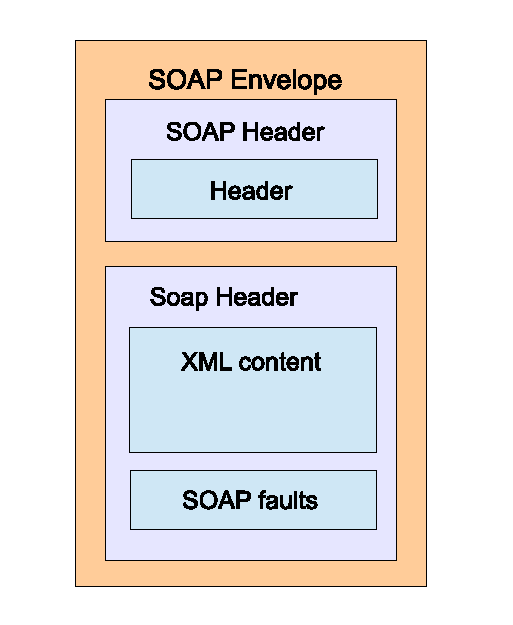
\includegraphics[width=0.5\textwidth]{figs/soap_structure.eps}
	\caption{ Les éléments d'un message \textsc{SOAP}}
	\label{fig:soap_structure}
    \end{subfigure}    

    \begin{subfigure}[b]{1\textwidth}
	\centering
	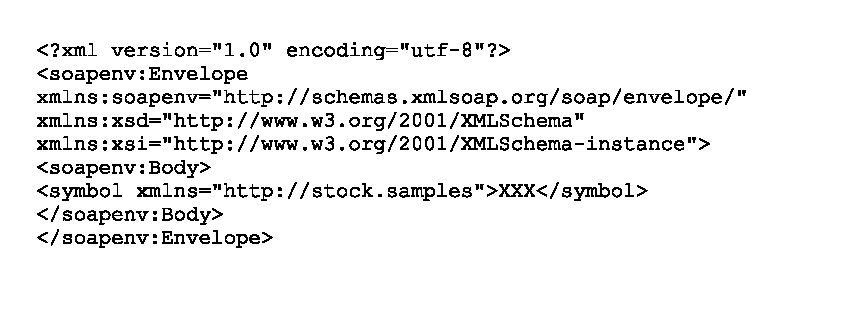
\includegraphics[width=1\textwidth]{figs/soap_message.eps}
	\caption{Exemple de message SOAP}
	\label{fig:soap-message}

    \end{subfigure}
    \caption{La structure d'un message \textsc{SOAP}}
    \label{fig:soap_all}
\end{figure}
 %% La structure d’un message SOAP
      Ce protocole \textsc{SOAP} est basé sur \textsc{XML} pour mettre en place
      un mécanisme valable d'échange des données indépendant du modèle de
      programmation de l'application et du système d’exploitation.
      
      Un message \textsc{SOAP} est un document XML constitué d'une enveloppe
      \textsc{SOAP} obligatoire, d'un en-tête \textsc{SOAP} facultatif et
      d'un corps \textsc{SOAP} obligatoire:

      % TODO pick something real from the app.  go to the annexes part
      % \begin{figure}[h]
    \begin{Verbatim}[frame=single, fontsize=\scriptsize]
	<?xml version="1.0" encoding="utf-8"?>
	<soapenv:Envelope
	xmlns:soapenv="http://schemas.xmlsoap.org/soap/envelope/"
	xmlns:xsd="http://www.w3.org/2001/XMLSchema"
	xmlns:xsi="http://www.w3.org/2001/XMLSchema-instance">
	<soapenv:Body>
	<symbol xmlns="http://stock.samples">XXX</symbol>
	</soapenv:Body>
	</soapenv:Envelope>
    \end{Verbatim}
    \caption{Exemple de message SOAP}
    \label{fig:soap-message-example}
\end{figure}



      % TODO SOAP message structure
      % \begin{figure}
      %   \centering
      % \end{figure}

      \SpecialItem
      \begin{description} % SOAP components
      \item[Enveloppe]: L'élément racine du message \textsc{SOAP} ,
        définissant le contexte du message, son destinataire et son contenu,
        il englobe l'en-tête et le corps.
        
      \item[En-tête \texttt{<Header>}]: Un mécanisme générique permettant
        d'ajouter des fonctions à un message \textsc{SOAP} d'une manière
        modulaire sans accord préalable entre les parties en communication.
        Des exemples d'extension qui peuvent être implémentées comme des
        en-têtes sont des authentifications, des transactions, des paiements
        
      \item[Corps \texttt{<Body>}]: Contient les informations obligatoires
        destinées à l'ultime destinataire du message, il sert comme un
        container pour les informations mandataires à l'intention du
        récepteur du message.  \textsc{SOAP} définit un élément pour le
        corps, qui est l'élément \texttt{<Fault>} (Erreur) utilisé pour
        rapporter les erreurs.
      \end{description}

      \subsubsection{Description: WSDL} %TODO rewrite
      Le langage de description des services Web \acrshort{wsdl}
      \cite{chinnici2007web} est une recommandation du \acrshort{w3c},
      maintenant dans sa deuxième version.  \textsc{WSDL} est basé sur
      \textsc{XML} pour décrire les fonctions opérationnelles de services
      Web. La description des\textsc{WSDL} sont composées d'un interface et
      des implémentations. L'interface est une définition abstraite et
      réutilisable service qui peut être référencée par plusieurs
      implémentations.
      % \begin{figure}[h]
   \begin{Verbatim}[frame=single, fontsize=\small]
	<description>
	    <interface>
		<operation>
		    <input
			messageLabel="xs:NCName"?
			element="union of xs:QName, xs:token"? >
			<documentation />*
		    </input>
		    <output
			messageLabel="xs:NCName"?
			element="union of xs:QName,
			xs:token"? >
			<documentation />*
		    </output>
		</operation>
	    </interface>
	</description>
    \end{Verbatim}

     % \caption{La représentation d'un élément Inteface}
    % \href{http://www.w3.org/TR/wsdl20/#eii-types}
    % \label{fig:wsdl20_interface}
\end{figure}



 TODO WSDL 2.0

      Le WSDL sert à décrire :
      % TODO
      \renewcommand{\labelitemi}{$\bullet$}
      \begin{itemize} % ce que WSDL offrire
      \item le protocole de communication (SOAP RPC ou SOAP orienté message)
      \item le format de messages requis pour communiquer avec ce service
      \item les méthodes que le client peut invoquer
      \item la localisation du service.
      \end{itemize}
      % TODO reference the section

      \subsubsection{Découverte: UDDI}
      \acrshort{uddi} \cite{clement2004uddi} est une standardisation pour la
      publication et la découverte des services Web initialement conçue et
      spécifiée par le Consortium de standards
      OASIS\footnote{\url{https://www.oasis-open.org}}, et il est le
      résultat d'un accord d'un ensemble d’industriels
      Ariba\footnote{\url{http://www.ariba.com/}}, IBM, Microsoft, etc en
      vue de devenir le registre standard de la technologie des services
      Web.

      \textsc{UDDI} complète les technologies basiques de services Web en
      permettant de créer un \textbf{annuaire} permettant de localiser sur
      le réseau le services web recherchés, les services référencés dans
      \textsc{UDDI} sont accessibles par l'intermédiaire du protocole de
      communication \textsc{SOAP}, et la publication des informations
      concernant les fournisseurs et les services doit être spécifiée en
      \textsc{XML} afin que la recherche et l'utilisation soient faites de
      manière \textbf{dynamique} et \textbf{automatique}.

      Un \textsc{UDDI} peut appartenir à un domaine public comme internet ou
      tout autre réseau accessible à un nombre non limité d’utilisateurs,
      comme il peut appartenir à un domaine restreint comme l'intranet d’une
      entreprise ou d'un groupe d'entreprise.
      % TODO UDDI discovery and binding example

      Les données stockés dans l'UDDI sont structurées (en \textsc{XML}) et
      organisées en trois parties connues:

      % TODO
      \begin{description} % les pages d'UDDI
      \item[Pages blanches]: fournissent des descriptions générales sur les
        fournisseurs de services à savoir le nom de l'entreprise qui fournit
        le service, son identificateur commercial, ses adresses, etc.
        
      \item[Pages jaunes]: comportent des descriptions détaillées sur les
        fournisseurs de services catalogués dans les pages blanches d'une de
        façon taxonomique (selon secteurs d'activités par exemple).
        
      \item[Pages vertes]: fournissent des informations techniques sur les
        services Web catalogués. Ces informations incluent la description du
        service, les adresses \textsc{URL}, du processus de son utilisation
        et des protocoles utilisés pour son invocation.
        
      \end{description}
      % TODO talks about:
          % OWL-S and why UDDI approach is semantically poor

      % TODO Conclure cette subsection par la mention du problème de la
      % découverte automatique des services Web et l'insuffisance de la
      % description syntaxique.

  \section{Description des services web}
  % \cite{sivashanmugam2003adding} \cite{mcilraith2003bringing}
  % \cite{vargas2009challenges} \cite{mcilraith2001semantic}
  % \cite{medjahed2004thesis}

  % TODO Refactore and eliminate some repetition TODO get more from
  % \cite{lopez2008selection}
  Une description du service Web est un document par lequel le
  fournisseur de services communique au client les spécifications pour
  invoquer le service Web, Dans cette section nous présentons les
  modèles de description des services web. Nous détaillons dans la
  première sous-section le modèle de description syntaxique
  \acrshort{wsdl} \cite{chinnici2007web} développé et standardisé par le
  \acrshort{w3c} qui est devenu un élément essentiel dans des
  technologies services web. Ensuite en mettant l'accent sur les
  limitations majeurs de cette approche dans un environnement hétérogène
  qui nécessite un certain degré de dynamisité et d'automatisation.
  Finalement, Nous présentons les divers approches sémantiques visant à
  préciser la description d'un service en insistant sur les approches
  d'annotation sémantique et sur les ontologies de services.

    \subsection{Description syntaxique de services}
    % TODO exoend this introduction and give some examples form a real
    % senario
    Le langage de description de services Web \acrshort{wsdl}
    \cite{chinnici2007web} fournit un modèle ainsi qu'un langage basé sur
    \textsc{XML} de description de services Web. Un fichier \textsc{WSDL}
    comprend une description des fonctionnalités d'un service, mais il ne
    se préoccupe pas de l'implantation de celles-ci.  Il contient aussi
    des informations concernant la localisation du service, ainsi que les
    données et les protocoles à utiliser pour l'invoquer. En pratique, le
    document \textsc{WSDL} \footnote{\url{http://www.w3.org/TR/wsdl20/}}
    est un document \textsc{XML} qui se divise en deux parties
    \cite{elie2010} :

    \SpecialItem
    \begin{itemize} % WSDL two main parts
    \item La définition \textbf{abstraite} de l'interface du service avec
      les opérations supportées par le service Web, ainsi que leurs
      paramètres et les types des données.
      
    \item La définition \textbf{concrète} de l'accès au service avec la
      localisation, par une adresse réseau du fournisseur de service
      \footnote{Service Endpoint}, et les protocoles spécifiques d'accès.
    \end{itemize}

    % TODO exemple pratique d'un document WSDL associé avec le document
    % SOAP de la section précédente
    Un document \textsc{WSDL} constitué de quatre éléments principaux
    \cite{chinnici2007web}: \texttt{<Types>}, \texttt{<Interface>},
    \texttt{<Binding>}, \texttt{<Service>}.

    \cite{baryannis2010} \cite{elie2010} \cite{lopez2008selection}
    \renewcommand{\descriptionlabel}[1]{\hspace{1.5cm}\texttt{#1}}
    \begin{description} % WSDL20 elements
      
    \item[<Types>]: L'élément \texttt{Types} sert à un conteneur
      définissant les données figurant dans les messages échangés par le
      service. \textsc{WSDL} supporte des types élémentaires prédéfinis
      (tels que les entiers, les chaînes de caractères et les dates). Si
      les données échangées possèdent une structure particulière, il est
      possible de les décrire à travers un schéma XML \cite{part20012}.
      
    \item[<Interface>]: Les interfaces\textsc{WDSL} offrent une manière
      abstraite de décrire la fonctionnalité du service, Contrairement à
      la représentation concrète offerte par les éléments de
      \texttt{<Bindings>} et de \texttt{<Services>} qui sera décrit plus
      tard.  Une interface \texttt{WSDL} est constitué d'un ensemble
      d'opérations, chacun d'entre eux décrivant d'une simple interaction
      entre le service et le client. Une opération décrit un séquence des
      messages d'entrées/sorties ou un modèle d'échange de message
      \footnote{message exchange pattern} suivie lorsque l'opération est
      invoqué. Pour chaque message contenu dans le motif
      \footnote{pattern}, un type de message est spécifié à l'aide des
      types qui ont été définis précédemment dans le document.
      \textsc{WSDL} contient huit modèles de messages prédéfinis, mais on
      peut facilement définir de nouveaux.
      % TODO refactor this part
    \item[<Binding>]: \cite{elie2010} \cite{baryannis2010} L'élément
      \texttt{Binding} reprend les opérations de l'élément
      \texttt{<Interface>} et leurs associe un protocole de transfert et
      des spécifications des formats de données de message.  La définition
      des protocoles de communication utilisés pour l'invocation du
      service Web permet d'établir le lien, d'une part, entre le document
      et les messages \textsc{SOAP} et d'autre part, entre les messages
      \textsc{SOAP} et les opérations invoquées.

      % A WSDL binding specifies concrete message format and
      % transmission protocol details
      % for an interface. Each operation in a WSDL description must
      % be associated with a
      % binding. Several typical binding extensions are defined in
      % WSDL 2.0 such as SOAP
      % binding or HTML binding, but the service provider is free to
      % use others provided that
      % they are supported by the client and the service
      % toolkits. The syntax for bindings
      % parallels the syntax of interfaces, since each interface
      % construct has a binding counter-
      % part. A binding can either be reusable, meaning that it is
      % applicable to any interface,
      % or not.

    \item[<Service>]: Cet élément définit la localisation du service Web
      décrit. Pour chaque interface décrite, un élément service lui est
      associé. Le sous-élément \texttt{<endpoint>} définit un port d’accès
      en référençant l’élément \texttt{<binding>} associé et en déclarant
      l'\textsc{URL} localisant le service (avec l’attribut
      \texttt{<address>}).

      % A WSDL service element specifies a single interface that the
      % service will support, and
      % a list of endpoint locations where that service can be
      % accessed. Each endpoint must
      % also reference a previously defined binding to indicate what
      % protocols and transmis-
      % sion formats are to be used at that endpoint. A service is
      % only permitted to have
      % one interface but there are workarounds for a service to be
      % able to expose multiple

      % précise l’adresse ou les adresses aux-quelles se trouve le
      % service. Un <service> est un ensemble
      % de <port>. Un <port> spécifie une adresse pour un <binding>
      % donné. Par exemple

      % Cet élément définit la localisation du service Web
      % décrit. Pour chaque
      % interface décrite, un élément service lui est associé. Le
      % sous-élément endpoint définit un
      % port d’accès en référençant l’élément binding associé et en
      % déclarant l’URL localisant le
      % service (avec l’attribut address). Ceci permet qu’une
      % interface d’un service possède plus d’une
      % localisation (i.e. plus d’un élément endpoint) pour répondre
      % aux problèmes d’indisponibilité.
    \end{description}

    \subsection{Ajout de la sémantique}
    % Pour pallier le manque de sémantique de WSDL, plusieurs approches
    % proposent de rajouter une couche au dessus de WSDL complétant la
    % description syntaxique par des précisions sémantiques.
    % \cite{lopez2008selection}
    Malgré les améliorations apportées au standard \textsc{WSDL} dans son
    deuxième version \cite{chinnici2007web}, la description du service
    reste uniquement au niveau fonctionnel, c'est-à-dire qu'elle contient
    la manière dont on peut utiliser le service et non ce que fait le
    service, le standard \textsc{WSDL} est limité à l'énumération des
    opérations et à la description des types des paramètres d'entrée et de
    sortie associés, elle ne caractérise pas la sémantique de la
    fonctionnalité accomplie par le service. Par conséquent, la
    description \textsc{WSDL} reste insuffisante lors du processus de
    sélection.  Pour pallier cette Difficulté, plusieurs approches
    proposent de rajouter une couche au dessus sémantique de \textsc{WSDL}
    complétant la description syntaxique par
    des précisions sémantiques.\\
    % explain the problem in the context if web services composition using
    % ...  \cite{bartalos2011effective}

    Dans un premier temps, on va essayer de clarifier la notion d'un
    services Web sémantique, puis étudie les langages émergeants qui
    permettent de décrire ce type de services Web.

      \subsubsection{Définition des services Web sémantiques}
      % TODO the semantic web stack in the appendix

      % la description syntaxique est insuffisante.  A Semantic Web service
      % is defined as an extension of Web service description through the
      % Semantic Web annotations, created in order to facilitate the
      % automation of service interactions . Therefore, from he perspective
      % of the functionality offered, Semantic Web services are still Web
      % services. The only difference lays in their description and the
      % consequent benefits that follow, namely the reduction of human
      % involvement in
      % he performed interactions.\\

      % What is semantic web?

      % Le Web tel que nous le connaissons aujourd'hui est encore conforme à
      % la vision initial

      % Le Web a été conçu principalement pour une utilisation par les
      % humains. Néanmoins, il existe un effort visant à automatiser son
      % utilisation et pour apporter le Web plus accessible pour les
      % machines

      % \cite{bartalos2011effective} The Web was primarily designed for use
      % by humans. Nevertheless, there is an ef- fort to automate its use
      % and bring the Web more accessible for machines. This has brought
      % forward the need for machine processable representations of
      % semantically rich information. This has brought forward the need for
      % machine processable representations of semantically rich
      % information: a vision at the heart of the Semantic Web

      L'objectif premier du Web sémantique est de définir et lier les
      ressources du Web afin de simplifier leur utilisation, leur
      découverte, leur intégration et leur réutilisation dans le plus grand
      nombre d'applications \cite{berners2001semantic}. Le Web sémantique
      doit fournir l'accès à ces ressources par l'intermédiaire de
      descriptions sémantiques exploitables et compréhensibles par des
      machines. En effet, Les technologies du Web sémantique complètent le
      Web actuel avec des outils sémantiques. Il ne s'agit donc pas de créer
      un nouveau Web ou un Web séparé de l'existant : ce Web de données
      repose entièrement sur les technologies et concepts qui ont fait le
      succès du Web tel que nous le connaissons aujourd'hui
      \cite{bertails2010web}.

      La réalisation du Web sémantique trouve ces racines dans le
      développement des langages de balisage inspiré par des travaux issue
      de la communié AI \cite{mcilraith2001semantic}, tels que \textsc{OIL}
      \cite{fensel2001oil}, \textsc{DAML+OIL} \cite{horrocks2002daml+oil} et
      \textsc{DAML+OTN} \cite{mcguinness2003daml} (ces deux derniers
      langages sont parties de la famille \acrshort{daml}).

      % TODO refactor
      Ces langaes ont une sémantique bien définies et permettent le balisage
      et la manipulation des taxonomique complexe et Des relations logiques
      entre les entités sur le Web. \cite{fensel2000creating}

      %!TEX root = ../main.tex
\begin{figure}[h]
    \centering
    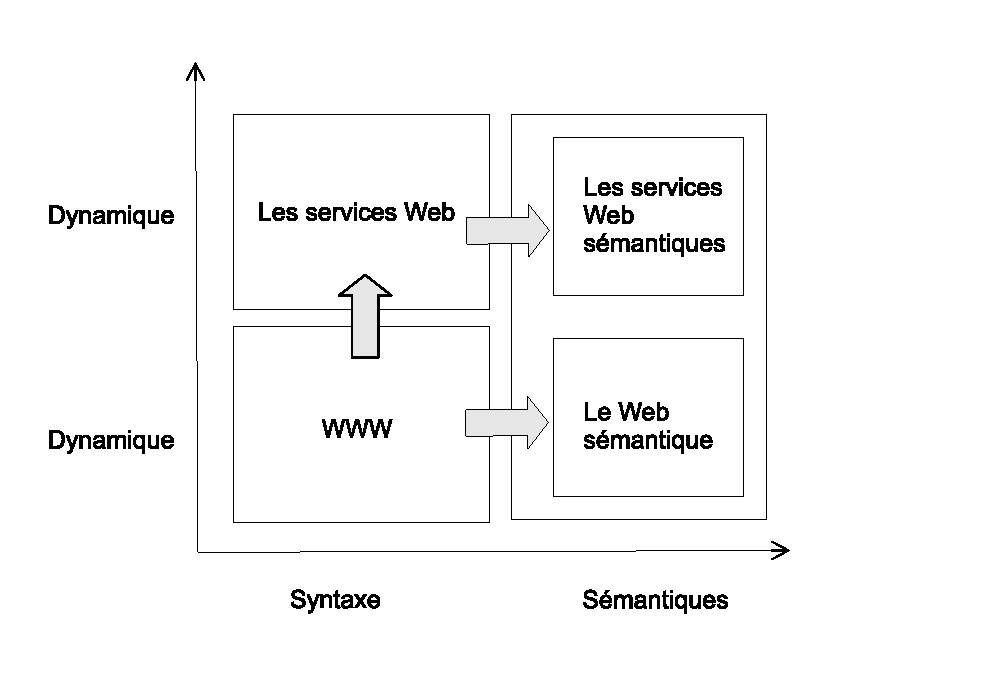
\includegraphics[width=1\textwidth]{figs/3w_to_sws.eps}
    %TODO translate
    \caption{Web evolution to Semantic Web services \cite{fensel2002semantic}.}
    \label{fig:3w_to_sws}
\end{figure}
      % \cite{lopez2008selection}
      Cette description repose sur des ontologies. Selon Gruber
      \cite{gruber1993translation}, une ontologie est une spécification
      explicite d'une conceptualisation. Une conceptualisation est un modèle
      abstrait qui représente la manière dont les personnes conçoivent les
      choses réelles dans le monde et une spécification explicite signifie
      que les concepts et les relations d'un modèle abstrait reçoivent des
      noms et des définitions explicites. Le Web sémantique est devenu un
      domaine à part entière, preuve en est la création en 2001 du groupe de
      travail sur ce sujet par le \textsc{W3C}.


      %  % Semantic web services
      % \cite{fensel2001oil}

      % What I need here ?  the base \cite{lopez2008selection}

      % \cite{berners2001semantic} % semantic web
      % \cite{bray1998extensible} % XML
      % \cite{part20012} % XML schema
      % \cite{lassila1999resource} %RDF
      % \cite{brickley2000resource} % RDFS
      % \cite{mcguinness2004owl} % OWL
      % \cite{decker2000semantic} % The semantic web: The roles of XML and RDF
      % \cite{gruber1993translation} % get ontologies def
      % \cite{uschold1996ontologies}
      % \cite{fensel2002web} % service semantic web between semantic web and the web services
      % \cite{mcilraith2003bringing} % Bringing semantics to web services
      % \cite{sivashanmugam2003adding} % Adding Semantics to Web Services Standards.

      % TODO define the nedeed for the semantic an example here will be nice
      % !  - insuffisance de description syntaxique des services web :(WSDL)

      % \subsubsection{Annotations sémantiques}
      % L'annotation sémantique consiste à enrichir et à compléter la
      % description d'un service\cite{elie2010}.  Elle établit des
      % correspondances entre des éléments de la description et des concepts
      % d'un ensemble d'ontologies de référence. Une ontologie de référence
      % permet de représenter un domaine par des structures interprétables
      % par une machine. Deux modèles principaux suivent l'approche
      % d'annotation sémantique, à savoir
      % \textsc{WSDL-S}\cite{akkiraju2005web}, \acrshort{sawsdl}
      % \cite{kopecky2007sawsdl}:
      % % et \textsc{METEOR-S} \cite{patil2004meteor}.

      % \renewcommand{\descriptionlabel}[1]{\hspace{1cm}\textbf{#1}}
      % \begin{description}
      % \item[WSDL-S]: C'est le résultat d'un travail collaboratif entre IBM
      %   et au laboratoire LSDSI. La spécification a devenue une
      %   recommandation \textsc{W3C} depuis 2005. Son objectif principal
      %   est de fournir un processus d'annotation sémantique compatible
      %   avec les technologies existantes. Pratiquement, Le méta-modèle
      %   \textsc{WSDL-S} repose sur les capabilités du modèle \textsc{WSDL}
      %   en rajoutant trois éléments majeurs \texttt{<category>},
      %   \texttt{<effect>} et deux deux attributs \texttt{modelReference}
      %   et \texttt{schemaMapping}. Les éléments introduits permettent de
      %   rajouter des informations qui n'étaient pas prises en compte dans
      %   \texttt{WSDL} comme \emph{les préconditions} et \emph{les effets}
      %   d'une opération. Tandis que les attributs permettent de référencer
      %   des concepts dans des ontologies de référence, ces préconditions
      %   et effets ensemble avec les annotations sémantiques des éléments
      %   \texttt{<inputs>} et \texttt{<outputs>} permet de l'automatisation
      %   du processus de découvert de services.

      %   TODO example of wsdl-s documeent \cite{elie2010}

      %   The WSDL [WSDL] document forms the anchor point for Web services
      %   description. Building on the descriptive capability of WSDL, we
      %   provide a mechanism to annotate the capabilities and requirements
      %   of Web services with semantic concepts referenced from a semantic
      %   model. To do this, we provide mechanisms to annotate the service
      %   and its inputs, outputs and operations. Additionally, we provide
      %   mechanisms to specify and annotate preconditions and effects of
      %   Web Services. These preconditions and effects together with the
      %   semantic annotations of inputs and outputs can enable automation
      %   of the process of service discovery.  TODO complete this list wit
      %   a real uses case with a sample wsdl-s document
      %   \begin{itemize}
      %   \item L'élément \texttt{<category>}
      %   \item \texttt{<precondition>}
      %   \item \texttt{<effect>}
      %   \item L'attribut \texttt{modelReference}
      %   \item \texttt{schemaMapping}
      %   \end{itemize}
      % \item[SAWSDL]:
      % \end{description}
      % \subsubsection{Ontologies de services}
      % Une ontologie de services saisit les différents aspects liés à la
      % description des services et leur utilisation à travers un ensemble
      % de concepts, de propriétés et de relations entre eux. Tois modèles
      % d'ontologies de services sont décrits ci-après \textsc{OWL-S}
      % \cite{martin2004owl}, \acrshort{wsmo} \cite{de2006web} et
      % \acrshort{swsf} \cite{battle2005semantic}:


      % \begin{description}
      % \item[OWL-S] \cite{mcilraith2003bringing}
      % \item[WSMO ]
      % \item[SWSF ]
      % \end{description}

      \subsubsection{WSDL-S}
      \textsc{WSDL-S} \cite{akkiraju2005web} est le résultat d'un travail
      collaboratif entre IBM, laboratoire LSDSI et l'iniversité de Geogia
      \footnote{\url{http://www.uga.edu/}}.  La spécification a devenue une
      recommandation \textsc{W3C} depuis 2005. Son objectif principal est de
      fournir un processus d'annotation sémantique compatible avec les
      technologies existantes. Pratiquement, Le méta-modèle \textsc{WSDL-S}
      repose sur les capabilités du modèle \textsc{WSDL} en rajoutant trois
      éléments majeurs \texttt{<category>}, \texttt{<effect>} et deux
      attributs \texttt{modelReference} et \texttt{schemaMapping}. Les
      éléments introduits permettent de rajouter des informations qui
      n'étaient pas prises en compte dans \texttt{WSDL} comme \emph{les
        préconditions} et \emph{les effets} d'une opération. Tandis que les
      attributs permettent de référencer des concepts dans des ontologies de
      référence, ces préconditions et effets ensemble avec les annotations
      sémantiques des éléments \texttt{<inputs>} et \texttt{<outputs>}
      permet de l'automatisation du processus de découvert de services.


      % TODO example of wsdl-s documeent \cite{elie2010} TODO complete this
      % list wit a real uses case with a sample wsdl-s document
      \begin{itemize} % WSDL-S elements and attributs
      \item L'élément \texttt{<category>}
      \item \texttt{<precondition>}
      \item \texttt{<effect>}
      \item L'attribut \texttt{modelReference}
      \item \texttt{schemaMapping}
      \end{itemize}

      \subsubsection{SAWSDL}	    
      La spécification \acrshort{sawsdl} \cite{kopecky2007sawsdl} est la
      suite de \textsc{WSDL-S} et il partage les mêmes principes de ce
      dernier. issue d'initiative du groupe de travail d'annotations
      sémantiques pour \textsc{WSDL} \footnote{Semantic Annotations for WSDL
        and XML Schema} et soumise au \textsc{W3C} en 2007, \textsc{SAWSDL}
      définit un mécanisme d'annoter sémantiquement les interfaces et les
      opérations \textsc{WSDL}, ainsi que les types \textsc{XML schema} en
      les reliant à des concepts dans une ontologie.  Cette annotation
      repose sur la définition d'attributs étendant le standard de
      description.  Les annotations sémantiques référencent des ontologies
      pré-existantes. Le mécanisme d'annotation de \textsc{SAWSDL} est
      indépendant de tout langage de représentation
      \cite{lopez2008selection} d'ontologies.

      \textsc{SAWSDL} propose deux sortes d'annotations sémantiques: une
      pour identifier le concept sémantique (représentée par l'attribut
      \texttt{modelReference}) et une autre pour faire le lien entre le
      concept et le document \textsc{WSDL} (représentée par les attributs
      \texttt{liftingSchemaMapping} et \texttt{loweringSchemaMapping}).
      % TODO add more about the sawsdl attributs from \cite{baryannis2010}
      % and \cite{elie2010}


      \subsubsection{OWL-S}
      % \cite{baryannis2010} \cite{elie2010} \cite{lopez2008selection}

      % \cite{mcilraith2003bringing} % Bringing
      % \cite{martin2004owl} %OWL-S
      % \cite{ankolekar2002daml} % daml-s
      % \cite{mcguinness2004owl} % OWL
      % \cite{paolucci2002semantic} %Semantic matching of web services capabilities
      \textsc{OWL-S} \cite{martin2004owl} désigné par \textsc{DAML-S} dans
      les versions antérieures \cite{ankolekar2002daml}, est un langage
      issue des travaux de la \acrshort{darba}
      \footnote{\url{http://www.darpa.mil/}} et son programme
      \acrshort{daml} \footnote{\url{http://www.daml.org/services/}} en
      collaboration avec des chercheurs de plusieurs universités et
      organisations (l'Université de Toronto, Yale, Nokia, etc.). Il a été
      intégré au consortium \textsc{W3C} en 2004, au sein du groupe
      d'intérêt sur les services Web sémantiques, lors de la recommandation
      du langage \textsc{OWL} \cite{horrocks2002daml+oil}
      \cite{mcguinness2004owl}.  Ankolekar \emph{et al.}
      \cite{ankolekar2002daml} présentent une ontologie pour les services
      web dans le but d'automatiser la \emph{découverte},
      \emph{l'invocation}, la \emph{composition} et la \emph{surveillance}
      de l'exécution des services \cite{mcilraith2003bringing}, les auteurs
      reprennent la notion de classes d'\textsc{OWL} et proposent
      l'ontologie \textsc{OWL-S}.

      %!TEX root = ../main.tex
\begin{figure}[h]
    \centering
    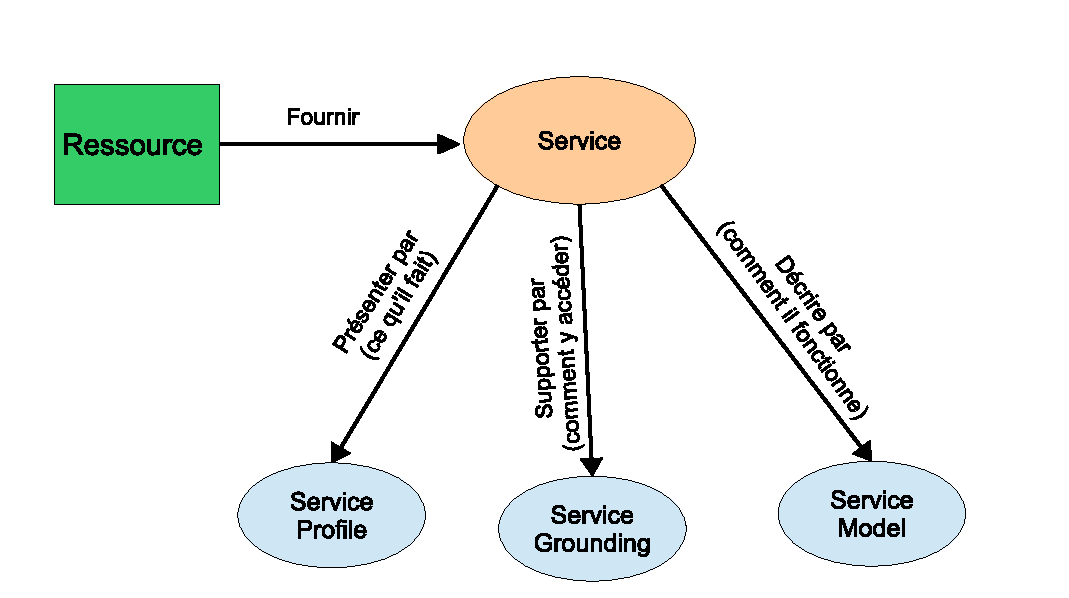
\includegraphics[width=0.8\textwidth]{figs/owls.eps}
    \caption{Les éléments d'une ontologie \textsc{OWL-S}}
    \label{fig:owl-s}
\end{figure}
 %TODO go for Tikz ✓

      L'objectif principal de ces recherches est d'établir une plateforme
      dans laquelle les descriptions des services Web sont partagés en
      utilisant une ontologie standard, constituée d'un ensembles de classes
      de base et des propriétés pour résoudre les ambigüités et de rendre la
      description d'un service compréhensible par une machine.

      la figure \ref{fig:owl-s} décrit la structure tripartie d'une
      ontologie \textsc{OWL-S}. Elle est composé de trois sous-ontologie: un
      \emph{service profile}, d'un \emph{service grounding} et d'un
      \emph{process model}.
      % TODO explain the fig:owl-s and add details about owls sub-ontologies
      \subsubsection{WSMO}
      \cite{baryannis2010}
  \section{Découverte des services web}
 % Description syntactique (UDDI) vs description sémantique

  % TOTANSLATE
  WS discovery is related to getting appropriate service for a request. It is one of the
  critical steps in the process of developing applications based on SOA. It can be done
  using syntactic matching or semantic matching\cite{Omer2011}.\\
  
  \section{Conclusion}
  % faire un petit récapitulatif sur les technologies des services web
  % rappeler de notre problème principale : composition des services web

%%% Local Variables: 
%%% mode: latex
%%% TeX-master: "../main"
%%% End: 

\chapter{La Composition des services web}
%% TODO Introduire la notion de la composition et le plan du chapitre

% Dans le chapitres précédent, nous avons étudiés la description, la
% publication,  la découverte et la sélection de services Web
% élémentaire. L'autre concept fondamentale % est la composition des
% services web.


  
%   % The other fundamental concept is web service composition which
% sometimes overlaps or will merge with the process of WS
% discovery. WS composition is a mechanism of combining two or more
% basic services into a possibly complex service. It is used to solve
% complex problems by combining available basic services. It helps to
% accelerate rapid application development and facilitate service
% reuse from developer perspective % and from user perspective it
% increases complex service consumption. As mentioned earlier a
% composite service can be regarded as a combination of services invoked
% in % a predefined order and executed as a whole and that has more
% functionality than its components. WS composition is needed because
% finding a right service provider for the request is not an easy task
% on fast growing WWW sometimes it is even % impossible. Thus WS
% composition becomes necessary and inevitable. Composing WS from
% existing ones is an effective method to fill this gap.\cite{Omer2011}

%   Dans ce chapitre, nous présentons dans un premier temps les
% définitions et les types de composition de services Web présents dans
% la littérature. Ensuite, nous étudions .....
%   Enfin, un ensemble de travaux proposent des approches de la
% composition dynamiques des services web sémantiques.

\newpage

  \section{Définition et stratégies de composition}
  \label{sec:defin-et-caract}

  Cette section a pour but d'exposer, d'une part, quelques définitions
  et objectifs de la composition des services Web proposées par la
  communauté, et d'autre part, les différents types et mécanismes de
  composition selon différents points de vue rencontrés dans la
  littérature.
  
    \subsection{Définitions}
    \label{sec:definitions}

    Martin \emph{et al.} \cite{martin2004owl} définissent
    la composition comme étant \emph{``le processus de sélection, de
      combinaison et d'exécution de services en vue
      d'accomplir un objectif donné''}.
    % TODO discussion de la définition.

    Selon S. Dustdar et W. Schreiner \cite{dustdar2005survey} :
    \emph{`` L'infrastructure de base des services Web suffit pour la
      mise en œuvre d'interactions simples entre un client et un
      service Web. Si la mise en œuvre d'une application métier
      implique l'invocation d'autres services web, il est nécessaire
      donc de combiner les fonctionnalités de plusieurs services
      web. Dans ce cas, nous parlons d'une composition de services
      Web''}.

    % TODO discussion.
    En d'autre terme, La composition de services Web désigne une
    opération qui consiste à construire de nouvelles applications ou
    services appelés \textbf{services composites} ou agrégats par
    l'assemblage ou l'agrégation de services existants nommés
    \textbf{services atomiques} ou élémentaires.

    Medjahed \cite{medjahed2004thesis}de ça part a défini un service
    Web composite commme un \emph{``conglomérat de sous-traitance
      services Web (services appelés participants) travaillant en
      tandem pour offrir un service à valeur ajoutée.''}\\

    La composition de services Web vise essentiellement quatre
    objectifs \cite{driss2011approche}:
    \begin{enumerate}
      \item Créer de nouvelles fonctionnalités en combinant des services
        déjà existants.
      \item Résoudre des problèmes complexes auxquels aucune solution\\
        n'a été trouvée.
      \item collaborer plusieurs entreprises ensemble.
      \item Optimiser et améliorer une fonctionnalité existante.
    \end{enumerate}

    % le processus générale de composition
    \subsection{Cycle de vie d'une composition }
    \label{sec:cycle-de-vie+exigences}
    % TODO: introduce
    % Dans cette sous-section, nous discutons du cycle de vie de la
    % composition de services Web, qui est divisé en quatre phases. Pour
    % chaque phase, un ensemble d'exigences est identifié.

    % Compte tenu de la nature très dynamique et distribué des
    % environnements de services Web, certaines exigences doivent être
    % respectées afin de parvenir à la composition de services Web
    % avec succès. Dans cette sous-section, nous identifions plusieurs
    % exigences pour chaque phase du cycle de vie d'un composition des
    % services Web.

    Comme l'illustre la figure, le cycle de vie de la composition de
    services Web comprend quatre phases \cite{sheng2014web}: la phase
    de \textit{définition}, La phase de \textit{sélection}, la phase
    de \textit{déploiement} et la phase d'\textit{exécution}:.

    \begin{figure}[h]
    \centering
    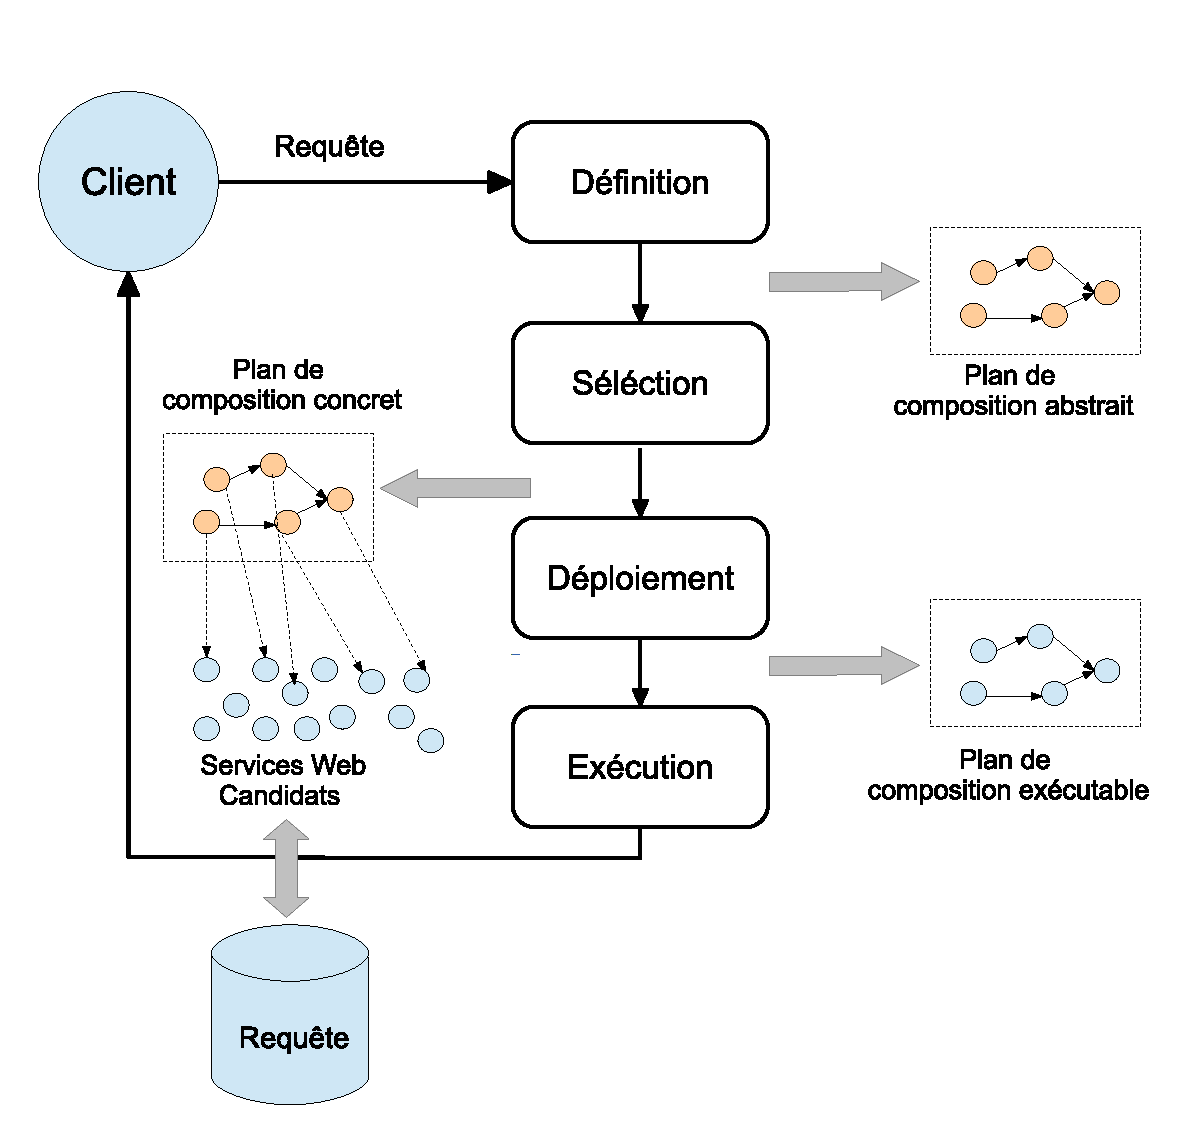
\includegraphics[width=0.9\textwidth]{figs/composition-life-cycle.eps}
    % TODO translate the figure
    % TODO reference the fig
    \caption{Cycle de vie d'une composition des services
      \cite{sheng2014web}.}
    \label{fig:composition-life-cycle.eps}
\end{figure}

%%% Local Variables:
%%% mode: latex
%%% TeX-master: "../main"
%%% End:
 \SpecialItem
    % \newpage
    \begin{description}
    \item[La phase de définition] Pendant cette phase, le client de
      service spécifie les exigence de composition des services en
      termes des besoins et des préférences pour le service
      composite. l'exigence est ensuite \textit{décomposé}, soit
      semi-automatique ou automatique, dans un modèle de
      \textbf{processus abstrait}(ce est à dire, le service composite
      abstraite), qui spécifie un ensemble d'activités, le contrôle et
      le flux de données entre eux, la qualité de service
      \acrshort{qos} et la gestion des exceptions.

      %% TODO: REWRITE
    \item[La phase de séléction.] Dans cette phase, pour chaque
      activité dans le service composite, les services Web appropriés
      qui répondent aux exigences de l'activité sont situés en
      cherchant sur le registre de service, sur la base des
      informations contenues dans les documents de description de
      service publiées. Il est probable que plus d'un service de
      candidat de répondre aux exigences. Par conséquent, le meilleur
      le service identifié doit être sélectionné. Après tous les
      services Web requis sont identifiés et liés aux activités
      correspondantes, le service composite construit est produite.

    \item[La phase de déploiement.]Dans cette phase, le service
      composite construit est déployé pour permettre son
      instanciation et l'invocation par les utilisateurs finaux. Le
      résultat de cette phase est le service composite exécutable.

    \item[La phase d'exécution.] Dans cette phase, l'instance de
      service composite est créé et exécuté par le moteur
      d'exécution, qui est aussi responsable de l'invocation des
      composants de service atomiques. Pendant l'exécution de
      l'instance de service composite, les tâches de surveillance, y
      compris le suivi d'exécution, mesure de la performance et la
      gestion des exceptions, doivent être effectuées.
    \end{description}
    \newpage
    \subsection{Procédés de coordination}
    \label{sec:proc-de-coord}
    % It should be noted that these models are not used exclusively:
    % one approach can implement more than one models at the same
    % time.\cite{baryannis2010} %% TODO: translate
    Nous distinguons deux méthodes utilisés pour décrire la
    composition de services dans un flot de processus métier:
    l'\emph{orchestration} de services et la \emph{chorégraphie} des
    services. Ces deux procédés de coordination décrivent deux aspects
    de création des processus métiers à partir des services Web
    composites \cite{peltz2003web}.
    %% Introduire la notion d'un procédé de coordination
    \textbf{Un procédé} est représenté par un graphe orienté
    d'activités ou un flot de contrôle qui donne l'ordre d'exécution
    des activités et la logique de coordination des services. Chaque
    activité représente une fonctionnalité réalisée concrètement par
    un service \cite{chollet2009orchestration}.

    La figure \ref{fig:orchestration-vs-choregraphie} illustre ces
    deux approches en conjonction.
    % orchestration vs chorégraphie
    \begin{figure}[h]
    \centering
    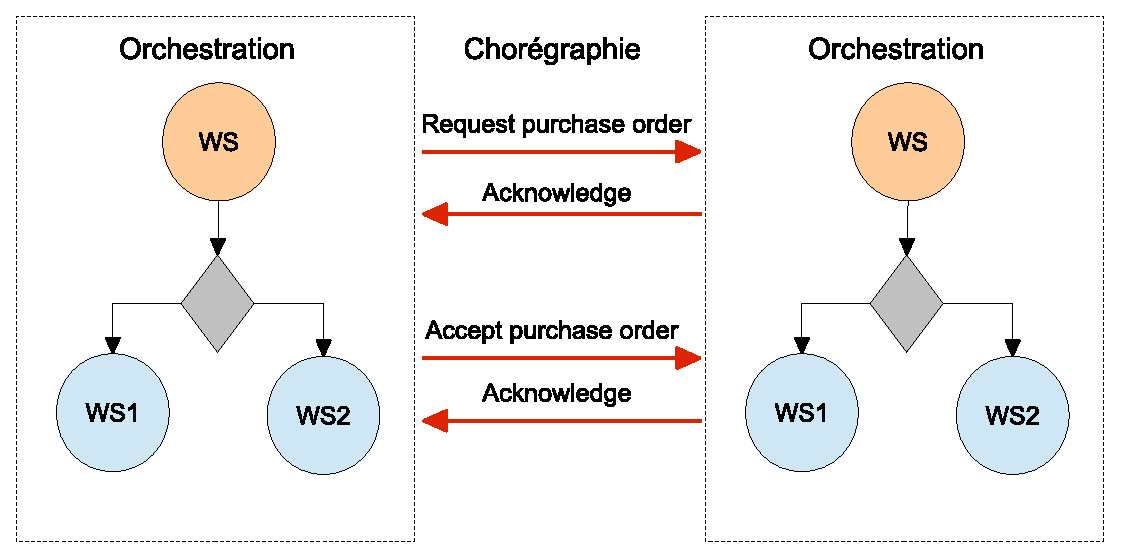
\includegraphics[width=1\textwidth]{figs/orchestration-vs-choregraphie.eps}
    \caption{Orchestration vs Chorégraphie selon Peltz
      \cite{peltz2003web}.}
    \label{fig:orchestration-vs-choregraphie}
\end{figure}       

      \subsubsection{Orchestration}
      \label{sec:orchestration-sec}
      Selon Sonia \emph{et al.} \cite{jamal2005environnement}:
      \emph{``L'orchestration des services Web permet de définir
        l'arranegement et l'enchaînement de ces services selon un
        canevas bien défini. Elle décrit la manière par laquelle les
        services peuvent interagir ensemble tout en incluant l'ordre
        d'exécution des différentes interactions''}.

      Barros \emph{et al.} \cite{barros2006standards} définissent
      l'orchestration comme un ensemble de processus exécutés dans un
      ordre prédéfini afin de répondre à un but
      \cite{lopez2008selection}. Ce type de composition se base sur un
      procédé métier exécutable permettant de décrire d'enchaînement
      et les interactions des différents services basiques collaborant
      dans une composition.
      
      L'orchestration offre \textbf{une vision centralisée} de
      contrôle, le procédé est toujours contrôlé par l'un des
      partenaires métiers. Ce dernier joue le rôle d'un chef
      d'orchestre qui se charge d'appeler les services de la
      composition suivant l'ordre d'exécution déjà défini par le
      processus métier. Le principe de l'orchestration est illustré
      par La figure \ref{fig:orchestration}.
      %TODO: citer qulques languages d'orchestration
      %TODO: les avantages et les inconvénients

      \subsubsection{Chorégraphie}
      \label{sec:choregraphie-sec}
      Selon Sonia \emph{et al.} \cite{jamal2005environnement} :
      \emph{`` La chorégraphie permet de tracer la séquence de
        messages échangés dans un contexte de composition de services
        Web. Elle est typiquement liée à la description de
        conversations existantes entre les services tout en impliquant
        plusieurs parties, incluant les clients, les fournisseurs et
        les partenaires''}.

      D'après Barros \emph{et al.} \cite{barros2006standards}, la
      chorégraphie permet de décrire la composition comme un moyen
      d'atteindre un but commun en utilisant un ensemble de services
      Web. La collaboration entre chaque service Web de la collection
      (faisant partie de la composition) est décrite par des flots de
      contrôle \cite{lopez2008selection}.

      La chorégraphie offre \textbf{une vision décentralisée} et
      \textbf{globale} du système et exprime une vue d'ensemble des
      services interagissant dans le cadre d'une composition de
      services. Selon Peltz \cite{peltz2003web}, la chorégraphie
      illustre les différants échanges de messages entre les
      participants. Le principe de la chorégraphie est illustré par la
      figure \ref{fig:choregraphie}.
      %TODO: citer qulques languages de chorégraphie.
      %TODO: les avantages et les inconvénients.

    \subsection{Stratégies de composition}
    \label{sec:types-de-composition}
    %TODO: re-write
    Un modèle de composition de service peut être relativement
    complexe. Il requiert la description et l'organisation de
    l'interaction entre les services et nécessite la gestion de
    plusieurs aspects comme les échanges de données entre les
    services, les pannes ou erreurs éventuelles, le contexte
    d'interaction, le degré d'automatisation des tâches, etc\dots
    
    Il existent une variété de spécifications, de langages et
    d'approches formelles développées par la littérature concernant la
    composition. Ces techniques sont également classés en fonction de
    différents dimensions, et selon les travaux effectués dans le
    champ des services web, les définitions des types de composition
    diffèrent d'une communauté de l'autre.
 
    Barros \emph{et al.} \cite{barros2006standards} classent la
    composition des services Web en trois catégories : la composition
    comportementale, l'orchestration et la chorégraphie, à l'instar de
    Barros \emph{et al.}, Peltz \cite{peltz2003web} considère que les
    deux dernières \textit{(orchestration, chorégraphie)}.

    \begin{figure}[h]
    \centering
    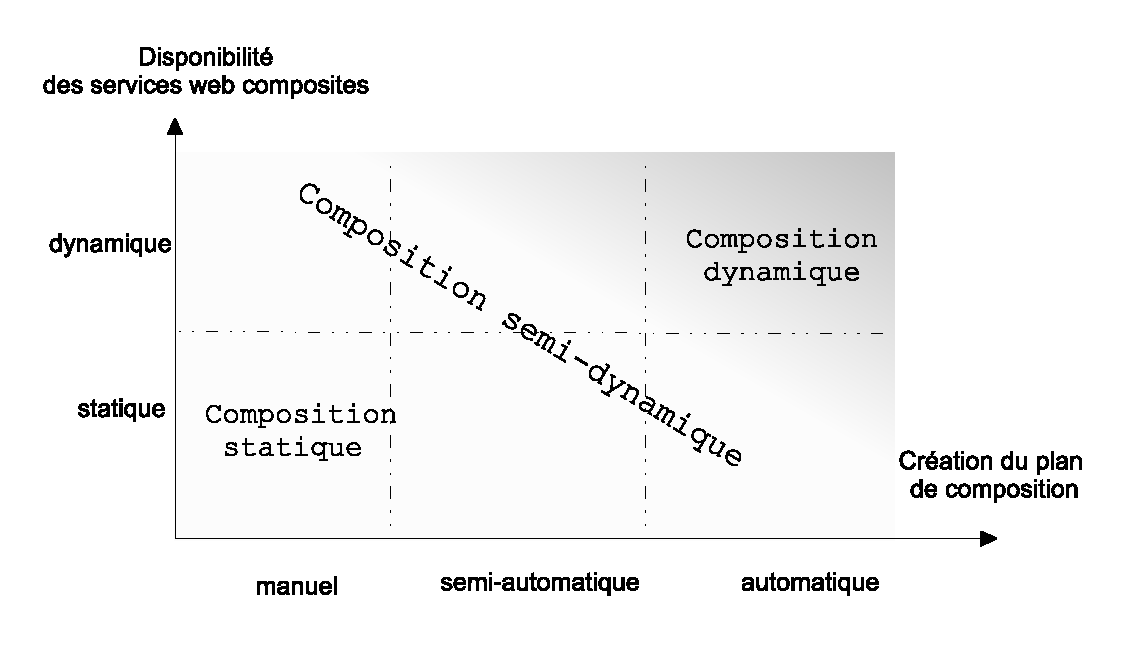
\includegraphics[width=1.1\textwidth]{figs/static-vs-dynamic-composition.eps}
    \caption{Classification des stratégies de composition
      \cite{fluegge2006challenges}.}
    \label{fig:static-vs-dynamic-composition}
\end{figure}
%%% Local Variables: 
%%% mode: latex
%%% TeX-master: "../main"
%%% End: 


    D'une autre façon, Fluegge \emph{et
      al.}\cite{fluegge2006challenges} dans une analyse de l'état de
    l'art considèrent l'orchestration et la chorégraphie comme des
    modèles d'exécution appliqués dans le contexte d'une
    composition. Il distingue trois stratégies de composition selon la
    disponibilité des services Web composites lors de composition et
    de le dégré d'automatisation: composition \textbf{statique},
    \textbf{semi-dynamique} et \textbf{dynamique} (voir la
    figure \ref{fig:static-vs-dynamic-composition}).

    %% Les Procédés de coordination comme une vision (point de vue)
    %% d'une composition des services Web.
    
    % Microsoft Biztalk et Bea WebLogic sont deux exemples de moteurs
    % de composition statiques de services Web. Pour la composition
    % dynamique, nous trouvons les plate-formes e-flow de HP et Sword
    % de Stanford.

    % Dans le cadre d'une composition statique de services, si les
    % fournisseurs proposent d'autres services ou changent les anciens
    % services, des incohérences peuvent être causées. Ceci qui
    % demande un changement de l'architecture du logiciel, voire de la
    % définition de l'application et crée l'obligation de faire une
    % nouvelle conception de l'application. C'est pourquoi, la
    % composition statique des services web est considérée rigide et
    % trop ee restrictive [86 S. Sanlaville, Environnement de proc ́d ́
    % extensible pour l'orchestration : Application aux services e e
    % web, Ph.D. Thesis, 2005 ]
    % \cite{driss2011approche}

      \subsubsection{Composition statique/dynamique}
      \label{sec:comp-stat}
      Selon la disponibilité des services composites, La composition
      des services Web peut être soit une composition statique soit
      une composition dynamique \cite{driss2011approche}:

      \SpecialItem
      \begin{description}
      \item[Composition statique] :est appelé aussi composition
        \textit{off-line}, précompil ou encore proactive. c'est une
        composition qui utilise des services basiques qui sont au
        préalablement définis d'une façon figée et qui ne peuvent pas
        changer en fonction du contexte du client. Ce type de
        composition engendre des applications peu flexibles, parfois
        inappropriées avec les exigences des clients.

        % Permet de créer de nouveaux services composites à partir des
        % services déjà existants dans des environnements « stables » où
        % les services Web participants sont toujours disponibles et où
        % le comportement du service composite est le même pour tous les
        % clients. La composition des services web prend place durant la
        % période de conception. Les composants sont choisis, reliés
        % entre eux et enfin compilés et déployés. Le service composite
        % ainsi obtenu fonctionnera bien tant que son environnement et
        % les services qui le composent ne changent pas ou ne changent
        % que rarement. Microsoft BizTalk est un exemple de moteurs de
        % composition statique. Ce type de composition est utile pour
        % mettre en place des services composites qui implémente des
        % services métiers connus et très souvent sollicités dans un
        % domaine donné (donc communs à plusieurs utilisateurs), par
        % exemple : achat d’un véhicule, planification d’un voyage...etc
        % . C'est d'ailleurs la raison pour laquelle ces approches se
        % limitent à un schéma d'orchestration (ou de chorégraphie)
        % prédéfini pour décrire les besoins préalablement connus de
        % l'utilisateur.

      \item[Composition dynamique]: appelée aussi composition
        \textit{on-line}, postcompilée ou encore réactive. Elle se
        réfère à la sélection des services basiques à la
        volée. Autrement dit, la sélection des services basiques ne
        peut pas être définie à l'avance mais elle sera faite au
        moment de l'exécution en fonction des contraintes imposées par
        le client. Ceci permet d' élaborer différents scénario de
        composition qui offrent les mêmes fonctionnalités et qui
        tiennent compte de la dynamique de la situation du client.

        % Dans ce type, les services Web à composer sont déterminés lors
        % de l’exécution de la requête d’un client. Ils peuvent être
        % déterminés selon les contraintes de chaque client, la
        % disponibilité des services Web, ...etc. La composition
        % dynamique apparaît la plus intéressante d’une part,elle promet
        % d'être capable de faire face à un environnement très dynamique
        % dans lequel des services apparaissent et disparaissent
        % rapidement. La composition des services web implique : - La
        % découverte des « bons » services à composer selon les besoins
        % et la disponibilité des services.  - La dynamicité et la
        % flexibilité dans la composition de services Web.
      \end{description}            

      \subsubsection{Composition manuel/automatique}
      \label{sec:comp-manu}
      Classification basée sur le degré d'automatisation.

      \SpecialItem
      \begin{description}
      \item[Composition manuel]: Suppose que l'utilisateur gère la
        composition avec sa main, via un éditeur de texte et sans
        l'aide d'outils dédiés.

      \item[Composition semi-automatique]: C'est un pas en avant en
        comparaison avec la composition manuelle, dans le sens qu'elle
        fait des suggestions sémantiques pour aider à la sélection des
        services Web dans le processus de composition.

      \item[Composition automatique]: La composition automatique (ou
        encore dynamique selon \cite{fluegge2006challenges}) permet un
        développement plus rapide des applications à base de
        services. Elle consiste à préciser la requête d'un utilisateur
        sous forme d'objectifs à satisfaire. Un moteur de composition
        \textit{``intelligent''} choisit la comabinaison de services
        répondant à l'objectif décrit. Il génère la composition de
        service adéquate de manière transparente à l'utilisateur. Ce
        principe a interpellé plusieurs communautés de recherche
        travaillant dans le domaine de l'Intelligence Artificielle.
        \cite{elie2010}
      \end{description}

      % \SpecialItem
      % TODO introduire la classification \cite{fluegge2006challenges}
      % TODO introduire les procédés de coordination par
      % \cite{peltz2003web}
      % \ref{sec:lang-de-comp}...
      % Dans la suite, les types de composition des
      % services Web désigne types classés
      % par\cite{fluegge2006challenges}.
  % \newpage
  \section{Langages pour la composition}
  \label{sec:lang-de-comp}
  % TODO: an introduction to the section
  % TODO: re-draw figs an unify them
  Afin de supporter la composition de services Web, plusieurs langages
  de composition de services ont été proposés pour décrire et mettre
  en oeuvre une composition. Dans cette section on va faire un tour
  d'horizon de quelques standards et langages principaux rencontrés
  dans la littérature.
  % % TODO change the font of commands in BPEL et al....
    \subsection{BPEL}
    \label{sec:bpel}

    \acrshort{bpel} est une spécification du consortium OASIS
    \footnote{\url{https://www.oasis-open.org}}issue de la fusion des
    spécifications \acrshort{xlang} Microsoft
    \footnote{\url{http://www.microsoft.com}}et \acrshort{wsfl} d'IBM
    \footnote{\url{http://www.ibm.com}}, il hérite les
    caractéristiques d'un langage structuré en blocs de
    \textsc{XLANG}, ainsi que les caractéristiques d'un graphe direct
    de WSFL \cite{driss2011approche}.

    \textsc{BPEL} \textit{(appelé aussi \acrshort{bpel4ws} ou
      \acrshort{ws-bpel})} est le langage d'\textbf{orchestration}
    le plus utilisé dans l'industrie permettant la coordination des
    interactions entre l'instance du service composite et ses
    partenaires sous forme d'un schéma \acrshort{xml} \textit{(le
      script d'orchestration)}, il définit le processus,
    l'enchaînement et l'ordonnancement des actions qui seront
    exécutées par le moteur d'orchestration, agissant comme une
    machine virtuelle capable d'exécuter \textbf{le procédé métier}
    intéreptable de \textbf{coordination} \cite{chollet2009orchestration}.

    \textsc{BPEL} repose sur un modèle constitué d'activités de
    coordination qui peuvent être de deux types, les activités de base
    ou élémentaires comme l'invocation (invoke) d'un service,
    l'attente d'une réponse et la génération d'une réponse
    (\verb|reply|), et les activités composites permettant du contrôle
    du flot de données comme les séquences (\verb|sequence|), les
    exécutions en parallèle (\verb|flow|) et les branchements
    (\verb|switch|, \verb|if|).

    %% procédé abstraite vs exécutable Selon \cite{chollet2009orchestration}
    % WS-BPEL est un langage de procédés basé sur la technologie XML,
    % tout comme les autres standards des services Web. WS-BPEL permet
    % de construire des procédés interprétables et exécutables par un
    % moteur d'orchestration.

    % Les procédés peuvent être modélisés de deux manières :
    % – abstraite : seuls les échanges de messages entre les
    % différents participants sont spécifiés. Mais le comportement
    % interne de ces participants n'est pas explicité.
    % – exécutable : les activités du procédé sont ordonnées; les
    % partenaires impliqués sont identifiés ainsi que les messages
    % qui sont échangés. A ceci s'ajoute le traitement des fautes
    % et des exceptions pour les cas d'erreurs.
    \subsection{WS-CDL}
    \label{WS-CDL}
    % make a reference to [TODO: Kavantzas et al., 2005] selon
    % elie2010
    \acrshort{ws-cdl} est un langage de composition de services de
    type \textbf{chorégraphie} qui permet de décrire une vision
    \textbf{globale} des collaborations entre les services Web
    \cite{elie2010}, à l'instar des standards de services Web,
    \textsc{WS-CDL} est basé sur \textsc{XML}, il complète la
    description \acrshort{wsdl} des services Web afin de décrire les
    interactions entre les participants (les services Web) de la
    composition.

    \textsc{WS-CDL} reprend et développe la spécification
    \acrshort{wsci} décrivant les séquences ordonnées de messages
    impliquant plusieurs entités (services Web) engagés dans une
    composition visant à accomplir un objectif commun.

    \textsc{WS-CDL} consiste à définir un fichier XML décrivant une
    chorégraphie, il permet de \cite{elie2010}:
    \begin{itemize} % WSDL-S elements and attributs
      \item désigner les variables et les types de données échangées.
      \item décrire les  activités impliquées.
      \item décrire les structures illustrant les interactions entre
      les activités.
    \end{itemize}

    % En résumé WS-CDL permet de décrire les règles selon
    % lesquelles une collaboration doit avoir lieu. Il fournit une
    % structuration globale de l'interaction en fonction de
    % laquelle chaque participant décrit son processus métier et
    % par suite ses services. \cite{elie2010}

    %  WS-CDL (Web Service Choreography Description Language) est un
    %  langage issu des efforts de standardisation
    %  du groupe de travail du W3C portant sur la chorégraphie de
    %  services Web (Web Services Choreography Working
    %  Group52). L'objectif de ce langage est de décrire les relations
    %  entre les services Web lors d'une composition de type
    %  chorégraphie.

    %  WS-CDL est un langage de composition de services de type
    %  chorégraphie définissant des contrats multi-parties. L’avantage
    %  de ce langage est que la description des interactions (l’élément
    %  Choreography du Package) est réutilisable. Ceci permet de
    %  diminuer la charge de travail des concepteurs. L’inconvénient de
    %  WS-CDL est que même si l’élément Choreography est réutilisable,
    %  sa description reste lourde. Un service doit posséder autant de
    %  Package que de participations à des compositions. De plus, WS-CDL
    %  n’inclut pas pour le moment de sémantique. Des travaux, tels que
    %  [Kang et al., 2007a] et [Kang et al., 2007b], proposent d’étendre
    %  WS-CDL afin d’y intégrer de nouveaux concepts (tels que la
    %  gestion des erreurs et des exceptions ou la mise en œuvre d’un
    %  minuteur d’exécution de la composition).
    %  \cite{lopez2008selection}

    \subsection{WSMF}
    \label{sec:wsmf}    
    \acrshort{wsmf} \cite{fensel2002web}est un initiative européen
    pour fournir une plate-forme riche de modélisation décrivant
    plusieurs aspects de services web. Son objectif principale est de
    permettre le commerce éléctronique (\emph{E-commerce}) par
    l'application de web sémantique aux services Web.

    Le standard \textsc{WSMF} est centré autour de deux principes
    complémentaire:
    
    % \begin{itemize}
    % \item découplage fort de différents aspetcs des applications de
    %   commerce électronique an e-Commerce application.

    % \item a strong mediation service enabling Web services to
    %   communicate in a scalable manner.
    % \end{itemize}

    % WSMF. The Web Service Modeling Framework (WSMF) [23] is an
    % European initiative to provide a fully fledged modeling framework
    % for describing various aspects related to Web services. Its main
    % goal is to fully enable e-Commerce by applying semantic Web
    % technology to Web services. WSMF is centered on two complementary
    % principles: (1) a strong de-coupling of the various components
    % that realize an e-Commerce application, and (2) a strong mediation
    % service enabling Web ser- vices to communicate in a scalable
    % manner. WSMF consists of four main elements: ontologies that
    % provide the terminol- ogy used by other elements; capabilities
    % repositories that define the problems that should be solved by Web
    % services; Web services descriptions that define various aspects of
    % a Web service; and mediators that bypass interoperability
    % problems.  There are two main projects in WSMF: the semantic Web
    % enabled Web Services (SWWS) and the Web Service Modeling Ontology
    % (WSMO). SWWS provides a description framework, a discovery
    % framework, and a mediation framework for Web services, while WSMO
    % service ontology includes definitions for goals, mediators, and
    % Web services.

    \newpage
    \subsection{OWL-S}
    \label{sec:owl-s}

    \textsc{OWL-S} \cite{martin2004owl} désigné par \textsc{DAML-S}
    \cite{ankolekar2002daml} dans les versions antérieures, est un
    langage issue des travaux de \acrshort{darba}
    \footnote{\url{http://www.darpa.mil/}} et son programme
    \acrshort{daml} \footnote{\url{http://www.daml.org/services/}} en
    collaboration avec des chercheurs de plusieurs universités et
    organisations. Il a été intégré au consortium \textsc{W3C} en
    2004, au sein du groupe d'intérêt sur les services Web
    sémantiques, lors de la recommandation du langage \textsc{OWL}
    \cite{horrocks2002daml+oil} \cite{mcguinness2004owl}.  Ankolekar
    \emph{et al.}  \cite{ankolekar2002daml} présentent une ontologie
    pour les services web dans le but d'automatiser la
    \emph{découverte}, \emph{l'invocation}, la \emph{composition} et
    la \emph{surveillance} de l'exécution des services
    \cite{mcilraith2003bringing}, les auteurs reprennent la notion de
    classes d'\textsc{OWL} et proposent l'ontologie \textsc{OWL-S}.
    %% TODO redraw the picture
    %!TEX root = ../main.tex
\begin{figure}[h]
    \centering
    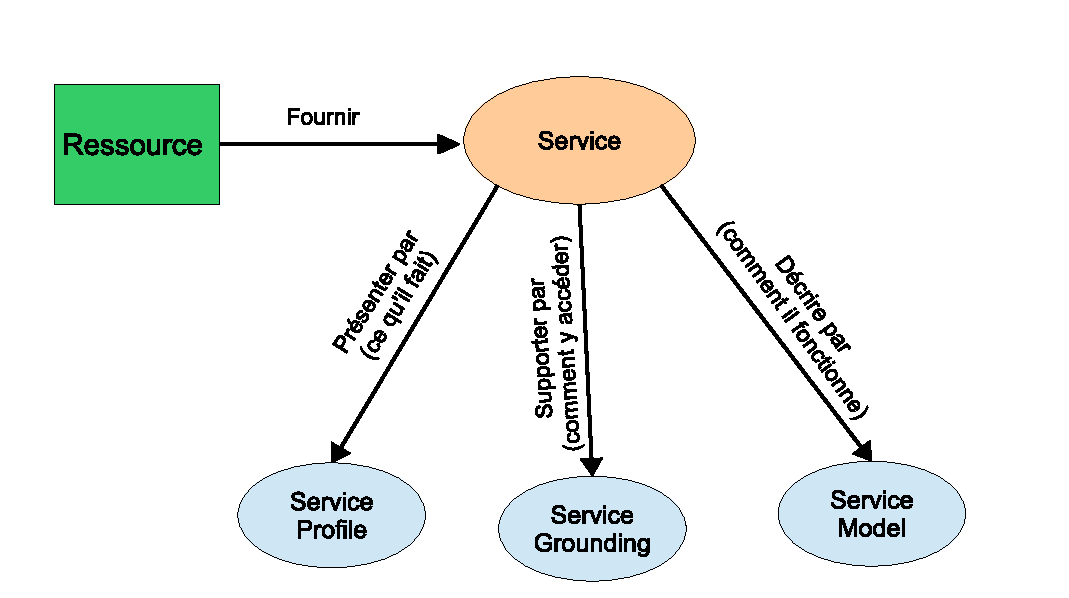
\includegraphics[width=0.8\textwidth]{figs/owls.eps}
    \caption{Les éléments d'une ontologie \textsc{OWL-S}}
    \label{fig:owl-s}
\end{figure}


    L'objectif principal de ces recherches est d'établir une
    plateforme dans laquelle les descriptions des services Web sont
    partagés en utilisant une ontologie standard, constituée d'un
    ensembles de classes de base et des propriétés pour résoudre les
    ambiguïtés et de rendre la description d'un service compréhensible
    par une machine.

    la figure \ref{fig:owl-s} décrit la structure tripartie d'une
    ontologie \textsc{OWL-S}. Elle est composé de trois
    sous-ontologie: un \emph{service profile}, d'un \emph{service
      model} et d'un \emph{service grounding}.

    \SpecialItem
    \begin{description}
    \item[ServiceProfile.] il offre une description informelle des
      fonctionnalités rendues par le service (\verb|serviceName|,
      \verb|textDescription|) et des informations concernant son
      fournisseur (\verb|contactInformation|). D'une aure côté, il
      spécifie des fonctionnalités offertes par le service (
      comportement fonctionnel) en terme de transformation
      d'information dénotée par les \textit{Entrés/Sorties}
      \textsc{(I/O)} (\verb|hasInput|, \verb|hasOutput|) et de
      changement d'état après l'exécution du service dénoté par les
      \textit{pré-conditions/effets} \textsc{(P/E)}
      (\verb|hasPrecondition|, \verb|hasResult|).

      Du point de vue de découverte et de la composition, Le
      \verb|ServiceProfile| est la partie la plus importante de la
      définition du service \textsc{OWL-S}.

    \item[ServiceModel.] il décrit le fonctionnement du service du en
      indiquant comment les résultats sont produits étape par étape
      précisant la façon un client peut interagir avec le service afin
      d'atteindre sa fonctionnalité. Ceci est fait en exprimant la
      transformation de données avec \textit{Entrés/Sorties}
      \textsc{(I/O)} etla transformation de l'Etat avec
      \textit{pré-conditions/effets} \textsc{(P/E)}.

      le \verb|ServiceProfile| est généralement considéré comme un
      sous-ensemble du \verb|ServiceModel|, contenant uniquement
      l'information nécessaire pour annoncer le service Web pour une
      découverte ultérieure.

    \item[ServiceGrounding.] Permet de spécifier les détails d'accès
      au service en précisant le protocole, le format des messages, la
      sérialisation et l'adressage. Il représente une correspondance
      \textit{(mapping)} entre la définition abstraite d'un processus
      \textsc{OWL-S} décrivant le service et la définition
      \textsc{WSDL} concrète des éléments nécessaires pour interagir
      avec le service.

      Le rôle de mise en correspondance est principalement à de
      combler l'écart entre la description sémantique des services Web
      (détallée dans le deux premières sous-ontologies) et les
      modèles de description de service existants qui sont
      principalement syntaxique (\textsc{WSDL}).
    \end{description}

    Le \verb|ServiceProfile| fournissent éventuellement d'autres
    informations supplémentaires sur le service comme la qualité
    qu'il assure en terme du temps de réponse et du coût, une
    classification possible d'un service \\(\verb|serviceCategory|),
    et un paramètre générique \verb|serviceParameter|.
    \\
    {\color{red}

      \SpecialItemi
      \begin{description}
      \item[Le processus atomique] directement invoqué par
        l’intermédiaire d’un Grounding
      \item[Le processus composé] décomposable en d’autres processus
        plus simples en utilisant les commandes de contrôle (par
        exemple : Si-Alors-Sinon, ...)

      \item[Le processus simple] non-invoquable, il fournit simplement
        une vue d’un processus atomique ou une représentation
        simplifié d’un processus composé.
      \end{description}

      Les composants principaux d’un modèle de processus sont
      l’ontologie de processus (Process Ontology) et l’ontologie de
      contrôle du processus (Process Control Ontology).  L’ontologie
      de processus, décrit un service en termes d’IOPE. Cette
      ontologie peut être utilisée afin de supporter l’invocation et
      la composition automatique de services web.  L’ontologie de
      contrôle de processus décrit chaque processus comme étant un
      état en prenant en compte son activation, son exécution et sa
      terminaison.

      Nous pouvons constater que le langage OWL-S s'adapte bien au
      besoin des méthodes de planification qui exigent une description
      de l’état du monde avant et après l’exécution d’un service donné.

      Any language is barely practical if its usage is not supported
      by tools. Several tools are proposed to create, or manipulate
      the OWL-S descriptions of services.  The most usable are OWL-S
      API, WSRF2OWLS, JAX-SA (Bab  et al., 2006, ık 2007; Habala et
      al., 2006). JAX-SA is an enhancement of WSRF2OWLS. The tool
      provides an interface on the top of the OWL-S API to create
      OWL-S service descriptions. The OWL-S generation process is
      semi-automatic. It requires a man- ually created configuration
      file depicting the mapping between the I/O parameters defined in
      WSDL and the ontological classes defined in OWL. Based on this,
      it automatically generates the semantic annotation. The
      disadvantage of all the tools is a lack of support to describe
      the pre-/post-conditions.\cite{bartalos2011effective}

      nous montrons dans la section suivante qu’elle présente des
      limitations pour en décrire les aspects non
      fonctionnels.\cite{jean2012prise}

      \begin{itemize}
        \item les limitaion de OWLS \cite{jean2012prise}
        \item d'augmentation de OWLS par QoS \cite{baryannis2010},
          \cite{kritikos2009requirements}
      \end{itemize}
    }


    \subsection{Comparaison}
    \label{sec:langs-comparaison}   
    % TODO review
    % les critères de comparaison
    Une composition des services Web nécessite la satisfaction de
    plusieurs exigences techniques (\cite{sheng2014web}
    \cite{bucchiarone2006survey}) , le tableau
    \ref{comparaison-des-standards-et-langages-d-composition} montre
    une comparaison entre les langages et standards étudiées dans
    cette section selon les critères suivants:
    \begin{table}[htb!]
  \centering
  \begin{tabular}{|lcccc|}
    \hline
    \head{Langages}& \textsc{BPLE} & \textsc{WS-CDL} & \textsc{WSFM} & \textsc{OWL-S}\\
    \hline\hline
    \textbf{Composabilité} &\verb|+|& \verb|+|&\verb|-|&\verb|+|\\
    \textbf{Representation du rôle} &\verb|+|& \verb|+|&\verb|-|&\verb|-|\\
    \textbf{Support des structures complexes} &\verb|+|& \verb|+|&\verb|-|&\verb|+|\\
    \textbf{Compensabilité} &\verb|+|& \verb|+|&\verb|-|&\verb|-|\\
    \textbf{Support du sémantique} &\verb|-|& \verb|-|&\verb|+|&\verb|+|\\
    % TODO réviser critères
    \textbf{Support industriel} &\verb|+|& \verb|-|&\verb|-|&\verb|+|\\
    \hline
  \end{tabular}
  \newline

  \raggedright
  (\verb|+|) support, (\verb|-|) pas du support.
  \caption{Comparaison des standards et langages de composition}
  \label{comparaison-des-standards-et-langages-d-composition}
\end{table}
%%% Local Variables:
%%% mode: latex
%%% TeX-master: "../main"
%%% End:


    \SpecialItem
    \begin{itemize}
      \item [La composabilité] indique la capacité
        d'assembler des services participants dans un processus de
        composition et de modéliser les interactions entre eux.

      \item [La representation du rôle] indique La représentation de
        rôle indique la capacité de refléter la le comportement que le
        participant doit présenter afin d'interagir dans le processus
        de composition.

      \item [Le support des structures complexes] la capacité de
        modéliser les structures complexes qui reflètent les règles
        des actions réalisées dans le processus de composition logique
        d'exécution et de commande.

      \item [Compensabilité] est la capacité de gérer les
        exceptions de processus lors de l'exécution du processus de
        composition

      \item [le support du sémantique] est la capacité de représenter
        la sémantique de services participants pour faciliter la
        découverte des services et la composition dynamique.

      \item [le support industriel] indiqué par la qualité des outils
        et le support industriel de la technologie.
    \end{itemize}
    % TODO expand the table here for more details + conclude this
    % subsection

    % gives a detailed language capacity comparison of BPEL, WS-CDL,
    % BPML, ebXML, OWL-S, and WSMF. From Table 1, we can see that all
    % languages except WSMF support the modeling of message exchanging
    % and complex structure. Only BPEL and WS-CDL have the comprehensive
    % expressibility to define interacting roles, complex structures,
    % exception handling and compensation management. BPML does not
    % support role representation and ebXML does not provide a
    % compensation mech- anism. We also can observe that only OWL-S and
    % WSMF provide semantic support for services composition.

    \section{Les approches de composition dynamiques des services web}
  \label{sec:comp-dynam}

  % {\color{red}
  %   \SpecialItemi
  %   References :
  %   \begin{itemize}
  %   \item[thesis:] \cite{bartalos2011effective},
  %     \cite{elie2010}. \cite{zahirathesis2008}, \cite{dumez2010approche}.
  %     \item[serveys:] \cite{baryannis2010}, \cite{rao2005survey},
  %       \cite{dustdar2005survey}.
  %   \end{itemize}
  %   \SpecialItemi }

  La littérature quit traite la problématique de composition des
  services comporte une multitude d'approches visant à décrire
  l'interaction entre les services afin construire de nouveaux
  services composites répondant à un objectif donné. Selon l'approche
  proposée, les interprétations différent de ce que devraient être
  traitées dans une approche de composition, Ils diffèrent également
  sur le degré d'automatisation impliqué dans le processus allant des
  approches semi-automatisées à entièrement automatisés.

  Dans cette section, nous allons décrire et classifier les approches
  principales de composition proposées par différents auteurs issues
  de plusieurs communautés de recherches. La classification présentée
  par la suite est basée essentiellement sur l'état de l'art fait par
  Baryannis \emph{et al.}\cite{baryannis2010}.

    \subsection{Les approches basées sur les workflow}
    \label{sec:les-approches-basees}

    \subsection{Les approches guidées par les modèles}
    \label{sec:les-appr-guid}
    \cite{dumez2010approche}

    \subsection{Les apprcohes mathématiques}
    \label{sec:les-apprc-math}
   
    \subsection{Techniques de planification}    
    \label{sec:techn-de-plan}
    Selon \cite{baryannis2010}, \cite{bartalos2011effective},
    \cite{chan2007survey}, \cite{peer2005web}, \cite{rodriguez2011automatic}

  \section{Conclusion}
  \label{sec:conclusion}
    % conclusion
  Introduire la composition dynamique basé sur le modèle graphe qui se
  sera détaillé dans le prochain chapitre.
  % TODO rapeller du problème initiale en contexte de ce chapitre en une
  % page
 

%%% Local Variables: 
%%% mode: latex
%%% TeX-master: "../main"
%%% End:

\chapter{Les approches de composition dynamique des services Web sémantiques baseés sur le modèle graphe}
%% Introduction to the chapter
\newpage
\section{Préliminaires}
% \section{Le processus de matching et la découverte des services Web sémantiques}
% positionner l'approche par graphe dans les classification déjà
% abordées

%   \subsection{Mésures de similarité}
%   \label{sec:mesure-de-similarire}
%   objectif des mesures de similarité sémantique est d'évaluer la
%   proximité sémantique entre les concepts (auxquels les termes des
%   requêtes et documents sont rattachés). Et comme le matching des
%   services web revient à trouver les similarités entre les concepts
%   décrivant les propriétés des services web, nous avons jugé utile
%   d’explorer les différentes méthodes de recherche de similarité
%   utilisées dans le domaine de la recherche d’information, en
%   particulier.
%   \begin{mydef}[Similarité entre concepts]
%     Une similarité $\sigma$: C $\times$ C $\rightarrow$ [0,1] est une
%     fonction de couples de concepts vers un nombre compris entre 0 et
%     1 exprimant le degré de similarité entre deux concepts, tel que:
%     \SpecialItemi
%     \begin{itemize}
%       \item x $\in$ C, $\sigma$(x,x) = 1
%       \item x, y $\in$ C, $\sigma$(x,y) = $\sigma$(y,x)
%     \end{itemize}
%   \end{mydef}
%   Les ontologies définissent les propriétés des concepts et les
%   relations entre concepts. Une de ces relations est utilisée dans
%   notre application est \textsc{is–a} (est-un). Cette relation est utilisée
%   pour extraire des taxonomies à partir des ontologies

%   \begin{mydef}[Similarité entre concepts]
%     Soit C l'ensemble de concepts définis dans une ontologie. On dit
%     que T est une taxonomie et on écrit T(C, $\leq$) tel que c $\leq$
%     c' signifie que c \textit{is–a} c' (le concept c est subsumé par
%     le concept).
%   \end{mydef}
%   De nombreuses approches ont été proposées pour évaluer la similarité
%   sémantique entre deux concepts. Ces approches se divisent en trois
%   catégories [Sli, 2006]: les approches basées sur les arcs, les
%   approches basées sur le contenu informationnel et les approches
%   hybrides. %% see annexe (1)
% \section{Matching des services Web sémantiques }
% \label{sec:match-des-serv-1}
% Le processus de matchmaking repose sur la recherche de similarités
% entre les paramètres descriptives de ces derniers. Il existe deux
% catégories de paramètres de description des services web: les
% paramètres fonctionnels et les paramètres non-fonctionnels que nous
% décrivons tout de suite.
%   \subsection{Les paramètres fonctionnels}
%   \label{sec:params-fonc}
%   La sémantique fonctionnelle décrit les fonctionnalités qu’offre le
%   service en terme de transformation d’information dénotée par les
%   Entrés/Sorties (I/O) et de changement d’état après l’exécution du
%   service dénoté par les pré-conditions/effets (ou post-conditions)
%   (P/E).  Ils sont appelés ainsi parce qu’ils sont nécessaires pour le
%   fonctionnement du service web. Ces paramètres sont utiles dans la
%   recherche des similarités. En effet, grâce au formalisme de
%   description des services web (OWL-S), on trouve une description des
%   données requises pour l’exécution du service (Inputs) et une
%   description des résultats obtenus après exécution (Outputs). D’un
%   autre coté, un service web peut altérer l’état du monde après son
%   exécution.  L’état du monde requis pour que le service s’exécute est
%   la pré-condition et le nouvel état généré après son exécution est
%   l’effet du service sur le monde. Par exemple le service de logging à
%   un site web possède comme information d’entrées le username et le
%   password et l’information de sortie est un message de
%   confirmation. Après l’exécution, l’état du monde change de
%   not\_logged\_in à logged\_in. Prenons un autre exemple, un transfert
%   d’argent du compte A vers le compte B ne peut se faire que si le
%   compte A est solvable (les pré-conditions).  Les effets décrivent
%   les sorties (Output) et l’impact d’une exécution d’un service
%   web. Tant dis que le terme post-condition focalise souvent sur la
%   description des conditions concernant les valeurs retournées des
%   opérations du service web. Dans notre exemple ci-dessus, un impact
%   de l'exécution serait le transfert réel de l'argent du compte de
%   carte de crédit pour le compte de destination alors que la
%   post-condition décrit qu'aucun argent ne s’est perdu lors du
%   transfert [Car, 2007].  L’opération de matching consiste alors à
%   relier les paramètres des différents services (faire correspondre)
%   entre eux et cela suivant des règles de correspondance.
%   \subsection{Les paramètres non-fonctionnels}
%   \label{sec:params-non-fonc}
%   Les paramètres non fonctionnels sont des paramètres qui ne sont pas
%   reliés directement aux fonctionnalités d’un service web, mais mesure
%   la qualité avec laquelle le service délivre ses
%   fonctionnalités. Parmi ces paramètres on trouve:
%   \SpecialItem
%   \begin{description}
%   \item [Le coût]: C’est une propriété non-fonctionnelle qui est
%     pertinente pour le client qui veut utiliser le service.
%   \item [La sécurité]: La sécurité est une propriété non-fonctionnelle
%     qui est pertinente à la plupart des services web. Elle applique
%     des aspects tels que la communication et le cryptage des données.
%   \item [La qualité]: La propriété qualité des services est un
%     ensemble de propriétés différentes qui affecte tous les aspects
%     spécifiques du service, son utilisation et sa production tel que
%     le temps de réponse d'un appel à une opération, la capacité du
%     service...etc
%   \end{description}
%   Le matching des paramètres non-fonctionnels des services web est
%   tout aussi important dans la phase de sélections des services
%   candidats. Les propriétés non-fonctionnelles sont typiquement
%   représentés comme des politiques de services web exprimées par le
%   langage WS- Policy [Car, 2007].
%   Généralement ces approches de matching des politiques peuvent être
%   utilisées pour l'optimisation et l’évaluation des plans de
%   composition.  Les services web correspondent à des entités
%   dynamiques. Ils peuvent devenir disponibles à tout moment de
%   l’exécution du système et découverts dynamiquement par leurs
%   clients. Les fournisseurs et les consommateurs de services doivent
%   donc disposer d’un moyen commun et fiable pour effectuer la
%   publication et la recherche de services. On entend par découverte
%   dynamique la possibilité de localiser automatiquement un ensemble de
%   services web, sélectionner un service spécifique qui répond à des
%   besoins particuliers de l’utilisateur.  Plusieurs initiatives ont
%   traité la problématique de la découverte des services web dont les
%   deux principales modèles suivants:
%   \subsection{Le modèle syntaxique de matching des services Web}
%   \label{sec:le-modele-syntaxique}
%   \subsection{Le modèle sémantique de matching des services Web}
%   \label{sec:le-modele-semantique}
%   \subsection{Graphe de dépendance}
%   \label{sec:graph-de-depandence}
%   \cite{Omer2011}

% TODO
% requirement for good web service composition

\newpage
\section{Travaux connexes}
\label{sec:travaux-relatives}
% TODO: une petite introduction aux travaux connexes

% La découverte d'un service composite à partir d'un graphe de
% dépendance consiste à trouver le meilleur chemin dans le graphe qui
% génère les sorties exprimées dans la requête. La recherche peut se
% baser sur l'optimisation d’une fonction d'utilité qui tient compte du
% degré de matching entre les services et aussi de la qualité de service
% qui peut être fournie par les services concrets. A cet effet, les
% méthodes de recherche du meilleur chemin de la théorie des graphes
% peuvent être exploitées.  Les méthodes de composition utilisant le
% modèle de graphe peuvent être classées en deux catégories selon que le
% graphe de dépendance soit construit à priori (en phase de publication
% des services) ou pendant le traitement de la requête de composition:

% Nacera (TODO: améliorer cette introduction)
% Certaines approches ont été proposées récemment pour la découverte
% dynamique d'un service composite à partir d'un graphe de service. En
% effet un graphe de service est généralement mis en place pour
% représenter les dépendances possibles entre les services en terme de
% flux de données (Entrées/Sorties). Cette dépendance est déterminée
% grâce à un mécanisme de matching (mise en correspondance) entre les
% services. Cette représentation permet d'exploiter certaines
% techniques en théorie de graphe pour la recherche du meilleur plan de
% composition.

% La découverte d'un service composite à partir d'un graphe de
% dépendance consiste à trouver le meilleur chemin dans le graphe qui
% génère les sorties exprimées dans la requête. La recherche peut se
% baser sur l'optimisation d'une fonction d'utilité qui tient compte du
% degré de matching entre les services et aussi de la qualité de service
% qui peut être fournie par les services concrets. A cet effet, les
% méthodes de recherche du meilleur chemin de la théorie des graphes
% peuvent être exploitées.  Les méthodes de composition utilisant le
% modèle de graphe peuvent être classées en deux catégories selon que le
% graphe de dépendance soit construit à priori (en phase de publication
% des services) ou pendant le traitement de la requête de composition

  \subsection{Génération Online du graphe de dépendance}
  \label{sec:generation-online}

  % liang2005and: AND/OR graph and search algorithm for discovering composite web services
  \begin{text}
    Dans \cite{liang2005and}, Liang \textit{et al.}  Présentent une
    formalisation du problème de composition de service comme un
    problème de recherche dans un graphe \textit{And/Or}. Donc un
    graphe de dépendance (SDG) est construit dynamiquement suite à une
    requête dans un domaine spécifique choisie par l'utilisateur. Un
    graphe \textit{And/Or} contient des nœuds et des connecteurs de
    deux types: connecteur And/connecteur Or.

    Un connecteur And reliant des services avec un autre service s'il
    existe une relation de type and entre les paramètres de ces
    services, càd, toutes les entrées fournis par les services doivent
    être disponibles pour l'exécution du service destinataire. Des
    services sont connectés par un Or avec un autre service s'il
    existe une relation logique de type Or entre les paramètres des
    ces services, càd, n'importe quel service pourra produire l'entrée
    requise par le service destinataire. C'est la caractéristique
    principale de cette approche: tenir compte des deux types de
    branchement \textit{And/Or}.  Après, un algorithme de recherche
    itératif est appliqué pour trouver le service composite minimal et
    complet satisfaisant la requête puis soumis à évaluation par
    l'utilisateur jusqu'à ce qu'il valide le résultat (méthode
    semi-automatique).

    % In 2005, Altheya Lang and Y.W.Su [5] presented a model for web
    % service composition based on AND/OR graph, and a graph search
    % algorithm for searching the graph to find out the composite
    % service(s) that satisfies a user request. For a given service
    % request that only can be fulfilled by a composition of web
    % services, their algorithm find the service categories that are
    % relevant to the request and dynamically create an AND/OR graph
    % to grasp the functional dependencies among the web services of
    % these service categories. The graph is changed based on the
    % information reflected in a request. The search algorithm is used
    % to search the changed AND/OR graph for a minimal and adequate
    % composite service template that satisfies the service demand.
    % The algorithm can be executed repeatedly on the graph to find
    % out different templates until the result is considered by the
    % service requester
  \end{text}

  % lecue2006formal: A formal model for semantic web service composition
  \begin{text}
    Dans \cite{lecue2006formal}, Freddy et Léger considèrent également
    l'existence d'un mécanisme de découverte des services candidats,
    puis établir toutes les relations de dépendance entre ces services
    en utilisant la notion de lien causal et sauvegarde des ces
    informations dans une matrice d'adjacence.

    % Optimizing qos-aware semantic web service composition
    % \cite{lecue2009optimizing}
  \end{text}

  % omer2009dependency Dependency based automatic service composition using directed graph
  \begin{text}
    Dans \cite{omer2009dependency}, les auteurs supposent que les
    services candidates avaient été déjà découverts localement par un
    algorithme de découverte orienté but. L'exécution du plan se déroule
    en quatre principales étapes.
    % \cite{Omer2011}

    \SpecialItem
    \begin{itemize}
    \item La première est la génération du graphe de dépendance grâce à
      un algorithme qui utilise une matrice d'adjacence des dépendances
      Inputs/Outputs \emph{}ntre les services. Les dépendances sont identifiés
      si au moins une paire de paramètre (des Input(WS1) et Output(WS2))
      sont en relation exact ou plug-in selon [Paolucci], càd, In(WS1)
      Out (WS2).

    \item La deuxième étape consiste à extraire du graphe les
      dépendances cyclique (de type Loop) en utilisant l'algorithme [4]
      puis régénérer un nouveau graphe de dépendance acyclique en
      remplaçant chaque sous- graphe cyclique par un nœud composé

    \item La troisième étape est l'extraction du plan de
      composition. Pour générer enfin le plan final, les nœuds composés
      seront remplacés par leurs sous-plans respectifs.
    \end{itemize}

    La principale contribution de ce travail est la manière de traiter
    les cas de boucle dans un graphe, ce problème particulièrement a été
    très peu abordé dans ce domaine.
  \end{text}

  % mahmoud2013towards: Towards a Graph-Based Approach for Web Services Composition
  \begin{text}
    Dans \cite{mahmoud2013towards} ... % TODO
  \end{text}


  \subsection{Génération Offline du graphe de dépendance}
  \label{sec:gener-offline}

   % intro
   \begin{text}
     certains auteurs considèrent qu'il serait plus intéressant
     d'utiliser des informations complètes sur tous les services
     publiés pour assurer une recherche plus exhaustive des services
     candidats à la composition. Pour cela, le graphe de dépendance
     est pré-généré à partir du registre ou sont publiés les
     services. Par conséquent, le graphe inclut toutes les dépendances
     possibles entre les services disponibles, par contre il peut être
     volumineux et doit être mis à jour au fur et à mesure des
     changements (l'arrivée ou non disponibilité des services).
   \end{text}

   % arpinar2005ontology: Ontology-driven web services composition platform
   \begin{text}
     Dans \cite{arpinar2005ontology}, ...
   \end{text}

   %hashemian2006graph: A graph-based framework for composition of stateless web services
   \begin{text}
     Dans \cite{hashemian2006graph} le graphe de depdendance est
     construit à priori dont les sommets représentent les paramètres
     (Inputs/outputs) et les arcs représentent les services (utilisant
     ces paramètres). Suite à une requête, le processus de composition
     se déroulera en deux étapes : a) trouver les services potentiels
     pouvant participer dans la composition en cherchant les sous
     graphes couvrant tous Ventrées et Vsorties (fournies dans la
     requête) en utilisant une recherche en largeur d'abords (breadth
     first search). b) La deuxième étape consiste à extraire les plans
     d'exécution en utilisant à partir des services découverts. Les
     structures de composition considérées dans ce travail sont les
     séquences, les branchements conditionnels.
   \end{text}

   %elmaghraoui2011graph: Graph based E-Government web service composition
   \begin{text}
     Dans \cite{elmaghraoui2011graph}, les auteurs modélisent à priori
     toutes les dépendances entre les services et aussi sauvegarde
     tous les meilleurs chemins entre les nœuds du graphe dans une
     matrice en utilisant l'algorithme de Floyed, en optimisant le
     degré de matching, temps d'exécution, coût et la disponibilité du
     service.
  \end{text}

  \subsection{Autres travaux basés sur le graphe matching}
  \label{sec:autres-travaux}
  Alfredo Cuzzocrea, Marco Fisichella: ‘A Flexible Graph-based
  Approach for Matching Composite Semantic Web Services’, 2011:
  modélise le service composite décrit dans OWL-S Process-Model sous
  forme d’un graphe orienté (modélise le flux de données+structure de
  contrôle) puis il fait le matching à deux niveaux avec la requête de
  l’utilisateur (suppose aussi que la requête fournit également le
  schéma de composition):

  - Matching des Inputs/Outputs de la requête
  à celle du service composite

  - Matching de la structure du service décrit dans la requête avec
  celle du service composite publié (la requête est aussi décrite sous
  forme de graphe) matching de pattern
  \newpage
  \subsection{Discussion et comparaison}
  \label{sec:discussion-comparaison}

  \begin{table}[htb!]
  \centering
  \resizebox{1.05\textwidth}{!}{%
    \begin{tabular}{|>{\centering\arraybackslash}m{1.5in}|>{\centering\arraybackslash}m{0.9in}|
        >{\centering\arraybackslash}m{1.6in}|>{\centering\arraybackslash}m{1in}|>{\centering\arraybackslash}m{1.4in}|@{}m{0pt}@{}}
      \hline
      \textbf{Approche}  & \textbf{Génération du graph} & \textbf{Algorithme utilsé}& \textbf{Sémantique} &  \textbf{Les paramètres non-fonctionnels} &\\
      \hline\hline %--------------------------------------------------------------------------------------------------
      % ---------------------------------------------------------------------------------------------------------------
      Liang \textit{et al.} \cite{liang2005and} & Online & Recherche dans un And/Or graph & Non & Non &\\ [6ex] %done
      \hline %\item ------------------------------------------------------------------------------------------------------
      Arpinar \textit{et al.} \cite{arpinar2005ontology}& Offline&Bellman-Ford& Oui & temps d'exécution &\\ [6ex] %done
      \hline %--------------------------------------------------------------------------------------------------------
      Freddy et Léger \cite{lecue2006formal} & Online &  &  &  &\\  [6ex]
      \hline %--------------------------------------------------------------------------------------------------------
      Hashemian \textit{et al.} \cite{hashemian2006graph} & Offline & Recherche en largeur d'abord (BFS) ou en profondeur (DFS) & Oui & Non&\\[12ex] %done
      \hline %-------------------------------------------------------------------------------------------------------
      Gu Zhifeng \textit{et al.} \cite{gu2008automatic}& Offline & Extension de And/Or graph utilisée par \cite{liang2005and}  & Non & Non &\\[12ex]
      \hline %--------------------------------------------------------------------------------------------------------
      Abrehet et Schill \cite{omer2009dependency}& Online & Variation d'une recherche topologique basée sur \cite{ma2007systematic}& Oui & Non &\\[12ex] %done
      \hline %--------------------------------------------------------------------------------------------------------
      Elmaghraoui \textit{et al.} \cite{elmaghraoui2011graph}& Offline & Extension de Floyd-Warshall & Oui & Coût, temps d'exécution, disponiblité.&\\[12ex] % done
      \hline %--------------------------------------------------------------------------------------------------------
      Samuel et Sasipraba \textit{et al.} \cite{samuel2011approach}& TODO & TODO & TODO & TODO&\\[10ex]
      \hline %--------------------------------------------------------------------------------------------------------
      Chaker Ben Mahmoud \textit{et al.} \cite{mahmoud2013towards} &Online & Non définie & Oui & Non &\\[6ex] %done
      \hline %--------------------------------------------------------------------------------------------------------
    \end{tabular}}
  \newline
  \caption{Comparaison des approches de composition basées sur le modèle graph}
  \label{comparaison-graph-composition}
\end{table}
%%% Local Variables:
%%% mode: latex
%%% TeX-master: "../main"
%%% End:

  % TODO
\newpage
\section{Vers les bases de données graphe}
\label{sec:vers-les-bases}

\section{Conclusion}
\label{sec:conclusion-2}

%%% Local Variables:
%%% mode: latex
%%% TeX-master: "../main"
%%% End:

\part{L'approche proposée}
\chapter{Une méthode de composition dynamique de services Web
  sémantiques utilisant Neo4j}
\label{ch:approche}

\section*{Introduction}
\addcontentsline{toc}{section}{Introduction} \markboth{INTRODUCTION}{}

\newpage
\section{Définitions préliminaires}
\label{sec:basic-defs}
Cette section à comme but d'introduire les notions de base ainsi que
les notations et terminologies \ref{sec:basic:ws} employées dans la
suite de ce chapitre, Ensuite nous présentons une formulation
mathématique de notre problème principale, à savoir, \textit{la
  composition des servies Web} sous forme d'un problème de recherche
du plus court chemin dans un graphe orienté
\ref{sec:basic:composition}.\medskip

  \subsection{Services Web}
  \label{sec:basic:ws}
  Chaque web service peut contenir les définitions de différentes
  opérations, identifiables par leur nom, leurs paramètres, Pour des
  raisons de simplicité, nous supposons que chaque service Web
  représente une seule opération.

  \begin{mydef}[\textbf{Service Web}]
    Un Service Web $S$ est un tuple $S = <I,O>$. $I/O$ désigne la
    liste des paramètres ``entrées/sorties'' où chaque paramètre est
    lié à un concept dans l'ontologie du domaine.
   \end{mydef}

  %!TEX root = ../main.tex
\begin{figure}[h]
    \centering
    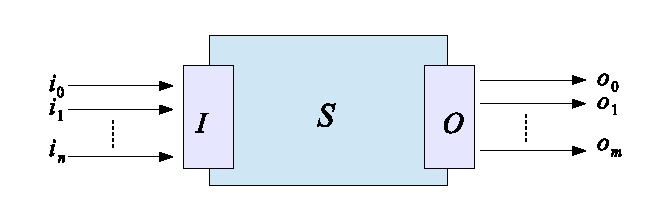
\includegraphics[width=0.7\textwidth]{figs/ch4/web-service.eps}
    \caption{Un service Web atomique.}
    \label{fig:ch4/web-service}
\end{figure}
%%% Local Variables:
%%% mode: latex
%%% TeX-master: "../../main"
%%% End:


  Nous pouvons donc définir un service comme une application $S$
  définie par:

   \[ S =
     \begin{cases}
       Inputs^n  \to Outputs^m \\
       (i_0, ..., i_n ) \mapsto (o_0, ..., o_m)\\
     \end{cases}
   \]\medskip

   $S$ possède $n$ paramètres d'entrée notés $i_0...i_n$ et $m$
   paramètres de sortie notés $o_0,...o_m$. Dans notre approche
   proposée, nous supposons que chaque service est décrit par un
   document \textit{OWL-S} où chaque paramètre (d'entrée ou de sortie)
   est lié à un concept dans une ontologie \textit{(OWL)} du domaine
   locale.\medskip


   Les ontologies de domaines locales sont les éléments essentiels des
   services web sémantique, créés par les prestataires de services. Un
   fournisseur a besoin de cette classe lorsqu'il crée un service web
   sémantique ainsi que leur ontologie de description (\textit{OWL-S})
   pour pointer les paramètres de ce service vers des entités de cette
   classe.

   \begin{mydef}[\textbf{Annuaire des services Web}]
     un annuaire des services $R$ (ou référentiel des services) est un
     ensemble $R =\{s_0, s_1, ...s_n\}$ des services Web disponibles
     qui peuvent être composés suite à une requête cliente de
     composition.
  \end{mydef}

  Dans notre l'architecture proposé, l'annuaire des services consiste
  à un service Web remplaçant un serveur \acrshort{uddi}. Ce service
  fourni l'ensemble des descriptions \textit{OWL-S} des services
  disponibles, chaque document référence un document \acrshort{wsdl}
  qui à son tour pointe vers l'\acrshort{url} de service décrit
  (\textit{Endpoint}), les descriptions sémantiques des services Web
  disponibles seront stockées dans une base de données relationnelle
  et exposées via un simple interface \acrshort{rest}.\medskip

  \begin{figure}[h]
    \centering
    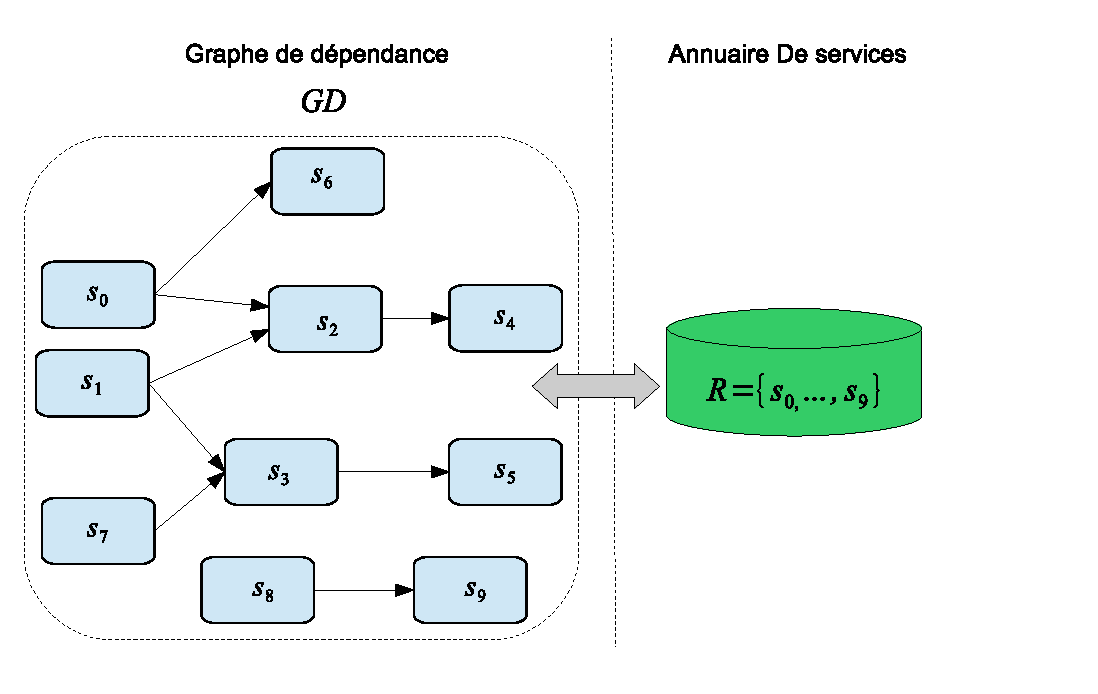
\includegraphics[width=1.2\textwidth]{figs/ch4/gd.eps}
    \caption{Graphe de dépendance $GD$ entre les services Web d'un
      annuaire $R$.}
    \label{fig:ch4/gd}
\end{figure}

%%% Local Variables:
%%% mode: latex
%%% TeX-master: "../../main"
%%% End:


  \subsection{Composition de services Web}
  \label{sec:basic:composition}
  Afin de découvrir et sélectionner un service Web composite suite à
  une requête cliente de composition, les services référencés dans un
  annuaire doivent être structurés dans un graphe orienté modélisant
  toutes les relations de dépendance fonctionnelle possibles réalisant
  un \textit{Matching} horizontal \ref{sec:ch4/matching} (la figure
  \ref{fig:ch4/gd}) entre les services disponibles deux par
  deux.\medskip

  \begin{mydef}[\textbf{Graphe de dépendance}]
    Un graphe de dépendance $GD$ est un ``graphe orienté et
    acyclique'' $GD=<R, E_r>$ qui modélise toutes les relations de
    dépendance fonctionnelle possibles entre les services Web
    disponibles dans un annuaire $R$. Il existe une relation $e=(s_0,
    s_1) \in E_r$ si et seulement si il existe une relation de
    dépendance entre $s_0$ et $s_1$.
  \end{mydef}

  L'approche proposée consiste à construire le graphe de dépendance à
  priori (\textit{Offline}) et le sauvegarder dans une base de donnés
  graphe (\textit{Neo4j}). Suite à une requête $Q$, un sous-graphe $G$
  est extrait reflétant un plan de composition exécutable $P$ d'un
  service Web composite satisfaisant.

  \begin{mydef}[\textbf{Requête}]
    Une requête $Q$ est un tuple $Q = <I', O'>$. $I'$ désigne la liste
    des paramètres d'entrée fournis par le client et $O'$ représente
    la listes paramètres requis (sorties).
  \end{mydef}

  \begin{figure}[h]
    \centering
    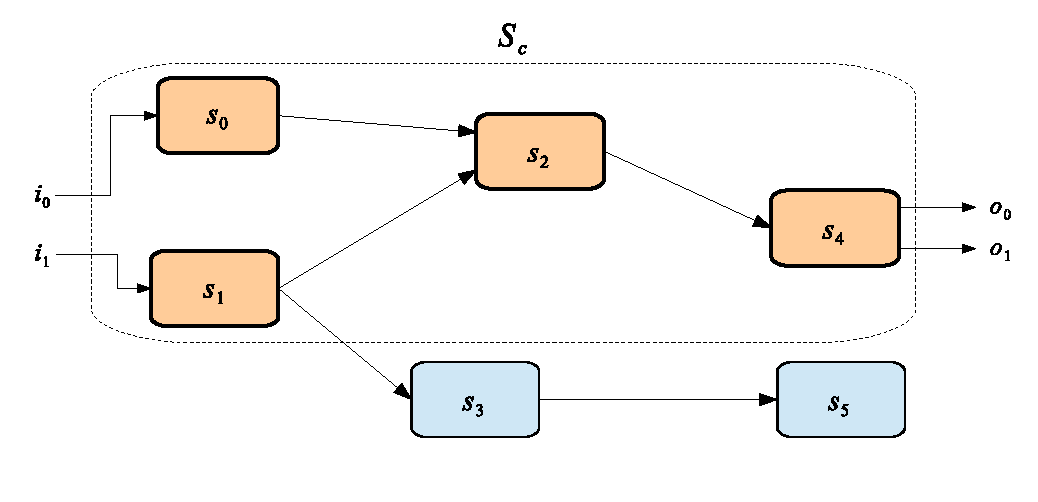
\includegraphics[width=1.1\textwidth]{figs/ch4/composition-plan.eps}
    \caption{Un service Web composite avec le plan de composition correspond.}
    \label{fig:ch4/composition-plan}
\end{figure}

%%% Local Variables:
%%% mode: latex
%%% TeX-master: "../../main"
%%% End:


  \begin{mydef}[\textbf{Plan de composition}]
    Un plan de composition $P$ est un sous-graphe
    $G$``\textbf{connexe''} d'un graphe de dépendance $GD$, $G=(V,E)$
    tel que $G \subset GD$ décrivant le flux de données/contrôles
    d'exécution d'un ensemble de services Web atomiques $V \subset R$
    engagés dans un processus de composition. Il existe une arête $e
    \in E$ tel que $e = (s_i, s_j)$ si l'exécution d'un service $s_j$
    dépend d'une ou plusieurs paramètres de sorties de $s_i$.
  \end{mydef}

  \begin{mydef}\label{def:ch4/sc}[\textbf{Service Web composite}] Un
    service Web composite $S_c$ est un service Web exécutable composé
    de ``$n$'' services atomique $s \in \{s_0,..., s_n\}$ tel que $n
    \succeq 1$, l'exécution d'un service Web composite correspond à
    l'exécution d'un plan de composition $P$ décrit par $G=<V,E>$ où
    $V = \{s_0, ..., s_n\}$ et $E$ décrivant les relations de
    dépendance entre les services $V$.
  \end{mydef}

  La figure \ref{fig:ch4/composition-plan} représente un service Web
  composite $S_c = <\{i_0, i_1\}, \{o_0, o_1\}>$ correspondant a un
  plan de composition $P$ représenté par un graphe\\ $G =<\{s_0, s_1,
  s_2, s_4\}, \{(s_0, s_1), (s_1, s_2), (s_2, s_4)\}>$.

\section{Matching des services  atomiques}
\label{sec:ch4/matching}

\section{Architecture proposée}
\label{sec:proposition}

\section{Construction et persistance du graphe de dépendance dans une
  base de donnée NeoJ}
\section{Découverte et exécution de services composites}

\section*{Conclusion}
\label{sec:conclusion}
\addcontentsline{toc}{section}{Conclusion} \markboth{CONCLUSION}{}


%%% Local Variables:
%%% mode: latex
%%% TeX-master: "../main"
%%% End:

\chapter{L'Implémentation d'un prototype}

\section{Example d'illustration}
\label{sec:example-dill-5}
\section{Outil d'annotaion sémantiques des services}
\label{sec:outil-dann-semant}
\section{Publication des services web atomiques}
\label{sec:atomic-publication}
\section{Découvert d'un service web composites}
\label{sec:composite-discovery}
\section{Conclusion}
\label{sec:Conclusion}

%%% Local Variables:
%%% mode: latex
%%% TeX-master: "../main"
%%% End:

\bibliographystyle{unsrt-fr}
\bibliography{references}
\begin{appendices}
\chapter{Le Web sémantiques}
% TODO appendix parts

% What is semantic web?

% Le Web tel que nous le connaissons aujourd'hui est encore conforme
% à la vision initial

% Le Web a été conçu principalement pour une utilisation par les
% humains. Néanmoins, il existe un effort visant à automatiser son
% utilisation et pour apporter le Web plus accessible pour les
% machines.

% \cite{bartalos2011effective} The Web was primarily designed for use
% by humans. Nevertheless, there is an ef- fort to automate its use
% and bring the Web more accessible for machines. This has brought
% forward the need for machine processable representations of
% semantically rich information. This has brought forward the need for
% machine processable representations of semantically rich
% information: a vision at the heart of the Semantic Web

Dans un premier temps, on va essayer de clarifier la notion d'un
services Web sémantique, puis étudie les langages émergeants qui
permettent de décrire ce type de services Web.

L'objectif premier du Web sémantique est de définir et lier les
ressources du Web afin de simplifier leur utilisation, leur
découverte, leur intégration et leur réutilisation dans le plus grand
nombre d'applications \cite{berners2001semantic}. Le Web sémantique
doit fournir l'accès à ces ressources par l'intermédiaire de
descriptions sémantiques exploitables et compréhensibles par des
machines. En effet, Les technologies du Web sémantique complètent le
Web actuel avec des outils sémantiques. Il ne s'agit donc pas de créer
un nouveau Web ou un Web séparé de l'existant : ce Web de données
repose entièrement sur les technologies et concepts qui ont fait le
succès du Web tel que nous le connaissons aujourd'hui
\cite{bertails2010web}.

La réalisation du Web sémantique trouve ces racines dans le
développement des langages de balisage inspiré par des travaux issue
de la communié AI \cite{mcilraith2001semantic}, tels que \textsc{OIL}
\cite{fensel2001oil}, \textsc{DAML+OIL} \cite{horrocks2002daml+oil} et
\textsc{DAML+OTN} \cite{mcguinness2003daml} (ces deux derniers
langages sont parties de la famille \acrshort{daml}).

  % TODO refactor
Ces langaes ont une sémantique bien définies et permettent le balisage
et la manipulation des taxonomique complexe et Des relations logiques
entre les entités sur le Web. \cite{fensel2000creating}

% %!TEX root = ../main.tex
\begin{figure}[h]
    \centering
    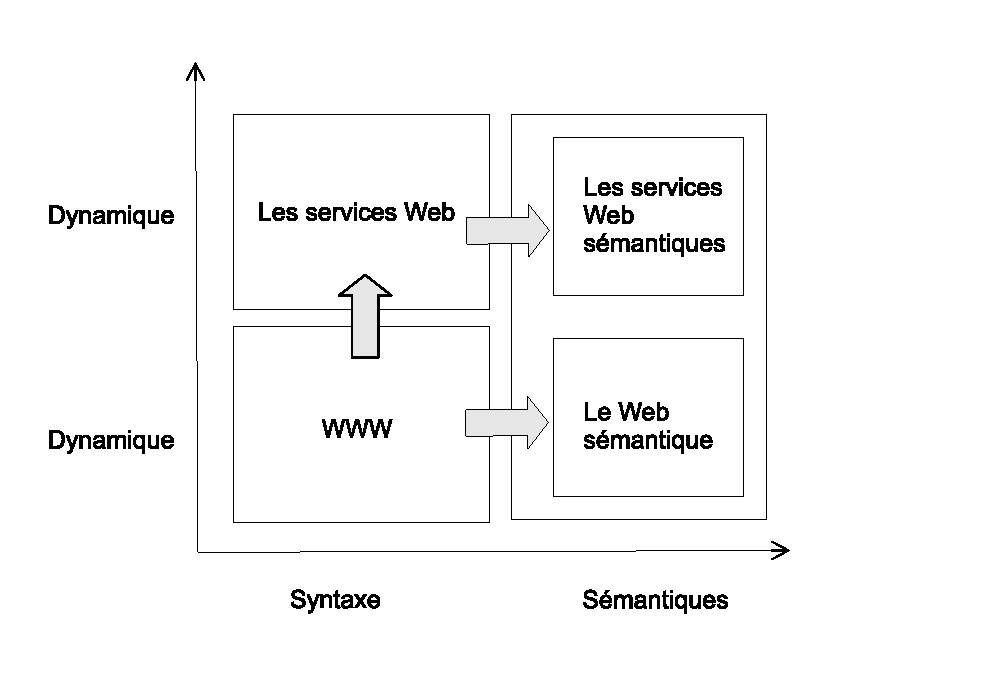
\includegraphics[width=1\textwidth]{figs/3w_to_sws.eps}
    %TODO translate
    \caption{Web evolution to Semantic Web services \cite{fensel2002semantic}.}
    \label{fig:3w_to_sws}
\end{figure}

Cette description repose sur des ontologies. Selon Gruber
\cite{gruber1993translation}, une ontologie est une spécification
explicite d'une conceptualisation. Une conceptualisation est un modèle
abstrait qui représente la manière dont les personnes conçoivent les
choses réelles dans le monde et une spécification explicite signifie
que les concepts et les relations d'un modèle abstrait reçoivent des
noms et des définitions explicites. Le Web sémantique est devenu un
domaine à part entière, preuve en est la création en 2001 du groupe de
travail sur ce sujet par le \textsc{W3C}.

%%% Local Variables: 
%%% mode: latex
%%% TeX-master: "../main"
%%% End: 

\end{appendices}

\end{document}

%%% Local Variables: 
%%% mode: latex
%%% TeX-master: t
%%% End: 
